\documentclass[a4, 12pt]{book}


%packages
\usepackage[english]{babel} %english language package
\usepackage[utf8]{inputenc}
\usepackage[T1]{fontenc}
\usepackage{amsmath} %math-mode package
\usepackage{amssymb} %math-mode package
\usepackage{wasysym} %astrological symbols package
\usepackage{xcolor} %color-package for text
\usepackage{mhchem} %nuclear notation package
\usepackage{ifthen} %logical operations for new commands
\usepackage{graphicx}
\usepackage{placeins} %Use for floatbarrier-function
\usepackage{listings} %for adding code
\usepackage{subcaption}
\usepackage{python} %use for python-environment
\usepackage{tikz}
\usepackage{geometry}
\usepackage{pdflscape}
\usepackage{hyperref}

%commands
\definecolor{myred}{rgb}{1,0,0}
\colorlet{MYRED}{myred} %for titles and such
\colorlet{Myred}{myred} %for titles and such 
\newcommand{\comment}[1]{ }%\textcolor{myred}{#1} }
\newcommand{\importantcomment}[1]{ {\Huge \comment{#1}} }
%\newcommand\todo{\comment{TODO!}}
\newcommand\todo[1][]{
        \ifthenelse{\equal{#1}{}}
                {\comment{TODO!}}
                {\comment{TODO! #1}}
}

%Packages and styles
\usepackage{natbib}
\bibliographystyle{../references/apj}
%\bibliographystyle{apalike}
%\bibliographystyle{dinat}
%\bibpunct{[}{]}{,}{a}{}{;}

%Citation commands
\newcommand\araa{ARA\&A}
\newcommand\aaps{A\&AS}
\newcommand\aap{A\&A}
\newcommand\apj{ApJ}
\newcommand\apjs{ApJS}
\newcommand\apjl{ApJL}
\newcommand\physrep{Phys.Rep.}
\newcommand\prc{Phys.Rev.C}
\newcommand\nat{Nature}
\newcommand\na{New Astronomy}
\newcommand\mnras{MNRAS}
\newcommand\mycite[1]{{\footnotesize \it \cite{#1}}}
\newcommand\mycitetwo[2]{{\footnotesize \it \cite[#2]{#1}}}

\newcommand{\isotope}[3]{
  \ifmmode {\ce{^{#3}_{#2}{#1}}}
  \else {\ce{^{#3}_{#2}{#1}}} \fi
}
\newcommand{\eu}[1]{\isotope{Eu}{63}{#1}}
\newcommand{\re}[1]{\isotope{Re}{75}{#1}}
\newcommand{\os}[1]{\isotope{Os}{76}{#1}}
\renewcommand{\u}[1]{\isotope{U}{92}{#1}}
\newcommand{\pb}[1]{\isotope{Pb}{82}{#1}}
\renewcommand{\th}[1]{\isotope{Th}{90}{#1}}
\newcommand{\w}[1]{\isotope{W}{74}{#1}}

\newcommand{\sos}{Solar system}
\newcommand\betadecay{$\beta^-$-decay }
\newcommand\betadecays{$\beta^-$-decays }
\newcommand\halflife{
  \ifmmode \tau_{\text{\tiny 1/2}}
  \else $\tau_{\text{\tiny 1/2}}$ \fi
}
\newcommand\msol{
  \ifmmode M_{\astrosun}
  \else $M_{\astrosun}$ \fi
}
\newcommand\omegamodel{\texttt{Omega}}
\newcommand\eris{\texttt{Eris}}
\newcommand\gasoline{\texttt{Gasoline}}
\newcommand\chemevol{\texttt{Chem\_Evol}}
\newcommand\sygma{\texttt{Sygma}}
\newcommand\nsm{neutron star merger}

%define lengths for subpages and subfigures
\newlength{\figwidth}
\newlength{\subfigwidth}

%define formatting for code-snippets
\definecolor{codegreen}{rgb}{0,0.6,0}
\definecolor{codegray}{rgb}{0.5,0.5,0.5}
\definecolor{codepurple}{rgb}{0.58,0,0.82}
\definecolor{backcolour}{rgb}{0.9,0.9,0.9}
\lstdefinestyle{custompython}{
    language=python,
    backgroundcolor=\color{backcolour},   
    commentstyle=\color{codegray},
    keywordstyle=\color{magenta},
    numberstyle=\tiny\color{codegray},
    stringstyle=\color{codepurple},
    basicstyle=\scriptsize,
    breakatwhitespace=false,         
    breaklines=true,                 
    captionpos=b,                    
    keepspaces=true,                 
    numbers=left,                    
    numbersep=5pt,                  
    showspaces=false,                
    showstringspaces=false,
    showtabs=false,                  
    tabsize=2
} %style for python-snippets


% Setting for layout
\setlength{\textwidth}{14.5cm}
\setlength{\headheight}{13.6pt}
\setlength{\marginparwidth}{0.7cm}
%\setlength{\marginparsep}{0.7cm}
\setlength{\evensidemargin}{1cm}


\newcommand{\mintittel}{Tittel}
\title{\mintittel}
\author{\O yvind Svendsen}
\date{01.06.18}

\begin{document}

\newcommand\supervisor{Supervisor: Sijing Shen\inst{1}}
\newcommand\cosupervisor{Co-supervisor: Signe Riemer-S{\o}rensen\inst{1}}
\newcommand\supervisors{\supervisor \\ \cosupervisor}
\DTMsavenoparsedate{presentationdate}{2018}{6}{15}{4}

\title{Modelling uncertainty of the Rhenium-Osmium cosmic clock}
\author{{\O}yvind Brynhildsvoll Svendsen\inst{1} \\[0.5cm] \supervisors}
\institute[Institute-opt-text]{ \inst{1} Institute of Theoretical Astrophysics, University of Oslo}
\date{\DTMusedate{presentationdate} \\ Svein Rosselands hus 209}
\subject{Astrophysics}

\frame{\titlepage}

\vspace*{18cm}
\noindent Copyright \copyright$\,$ 2018, \O yvind Svendsen
\vspace{4mm}

\noindent This work, entitled ``\mintittel'' is distributed under the
terms of the Public Library of Science Open Access License, a copy of which can be found at \url{http://www.publiclibraryofscience.org}. 

%\include{foreword}
%\include{acknowledgement}

%abstract
%introduction
\chapter{Introduction}
\chapter{Introduction}

After the big bang and the elements formed, the chart of nuclides was scarcsly filled.
Only the lightest elements and isotopes, hydrogen and helium primarily, filled the vast universe\cite{alphabetagamma}, in addition to the dark matter.
In the universe today we see much more heavier elements, and these must have been synthesised in some manner.
Nuclear fusion in stars create heavier elements up to iron, the heavier elements are made as by-products in which heavy atoms accumulates neutrons or protons and climb the chart of nuclides\cite{BBFH}.

Since \re{187} is shielded from the s-process, and \os{187} is shielded from the r-process, the synthesis of these isotopes are not
strongly coupled together. Granted, they both require heavy seed isotopes, hot neutron rich environments, and some method of ejection. The r-process needs so much higher neutron densities that it is believed to exist in vastly different stellar environments than the s-process\comment{(need some citation on the locations of r-process)}.
After \comment{insert halflife of re-187 here} half of \re{187} would have decayed to \os{187}, similar to the decay of \isotope{carbon}{6}{14} used in dating millenia old archelogical artifacts.
By taking the expected and observed abundance of the daughter and/or parent nuclei the age is determined by the ratio of isotopes and the halflife of the radioactive process.

By making a model of all the s-process and r-process sources in this Galaxy, the amount of synthesised \re{187} and \os{187} can be estimated. These estimates can be used to estimated the age of nucleosynthesis (when the heavy elements started forming).
Such a model is based on a mosaic of different scientific disciplines and data, and therefor also has a series of uncertainties from atomic properties to galactic history to numerical precision and everything in between. These uncertainties make the final image blurred.

This was attempted analytically by \comment{clayton + other articles} and they yielded \comment{value uncertainty from articles} and the results are useless compared to cosmological results \comment{add cosmological age of universe, galaxy etc} due to the huge uncertainties. However since the age of the Galaxy is known from cosmology, the biggest uncertainties in the synthesis-model can be constricted.

\section{Outline}

This thesis is divided into five chapters
\begin{description}
\item[Introduction]
\item[Theory I]
\item[Theory II]
\item[Results]
\item[Conclusion and discussion]
\end{description}

\comment{Explain [X/Y]}
\comment{introduce delay-time somewhere}


%theory I
\chapter{Theory Part I \comment{(need to rename)} }
\section{Cosmology}

\comment{Something something expansion}
\comment{Something something comiving coordinates}
\comment{Something something dark matter}
\comment{Something something baryonic matter}

\section{Nuclear physics}

\subsection{Nuclear shell model} \label{sec:nuclear model}
The atom is build up of electrons around a nucleus of protons and neutrons.
The electric coulomb forces keep the negatively charged electrons around the positively charged
protons in the nucleus. The protons and the neutrons are bound together by the strong nuclear force.
See figure \ref{img:atomic-structure} for illustration.

The quantum mechanical model of the atom is build up by quantum particles (electrons)
in the coulomb potential of the nucleus. The energy of the electrons is defined by their
radial quantum number, angular momentum quantum number, and intrinsic spin (analogous to
rotation about the particles own axis).

The strong force that holds the core together is not as well understood as the electric coulomb
force. In order to make a quantum mechanical model of the core it is assumed that all the
particles in the nucleus combined make up a central, harmonic potential. The protons and neutrons are
then modelled as quantum mechanical particles in the central field.
The states of the different particles is given by the principle quantum number $n$,
the orbital angular momentum quantum number $l$, and the total angular momentum quantum number $j=l\pm\frac{1}{2}$.
Similar to the aotmic model\mycitetwo{basdevant2005}{ch.2.4}.
The energy of these state do not stack linearly, but group together in a seemingly clumsy manners.
If particularly many energy states are grouped together, and the binding energy of nucleons peaks,
the group is called a magic number (see figure \ref{img:nuclear-shells}).

%Nuclear mass, binding energy, and reactions
\subsection{Mass and binding energy} \label{sec:binding-energy}
The total mass of the nucleus is given by the sum it's consituents, the nucleons.
Dividing by the mass number (number of nucleons in the core) one gets the average mass per nucleon.
This should be pretty elementary, but it turns out that the mass per nucleon dimishes
as mass number increases. Each proton and neutron becomes lighter as more protons and neutrons are stacked
into the central potential of the nucleus.
This energy is analogous to the energy needed to release nucleons from the nucleus potential\mycite{iliadis2015}.
See figure \ref{img:binding-energy-curve} to see how the average binding energy per nucleon evolves with number of nucleons in the nucleus.
\noindent
A classical example is two lighter nuclei colliding to one heavier nucleus. Since
the mass per nucleon is lower, but the total number of particles before and after has not changed the total
energy has lowered. This excess energy (or mass) is radiated away as thermal photons.
This implies that synthesizing heavier elements up to iron (peak binding energy in figure \ref{img:binding-energy-curve}) from
lighter elements releases energy.
Since protons and neutrons are fermions they follow the Pauli exclusion principle,
stating that a maximum of two particles can exist in any given quantum state in a bound system, and they must have opposite spins to do so\mycitetwo{basdevant2005}{ch.1.7.3}.
\noindent
E.g. Take a nucleus and continue to stack neutrons onto it, as the neutrons take on
higher and higher energy states (from the Pauli exclusion principle) the nucleus eventually reaches
a level where any new neutron would no longer be bound. The neutrons would therefore be immediately expelled.
If some protons were added, the strong force would be even stronger and more neutrons could be
added to the nucleus. The reverse is also true if protons were added continously.
This point in the nuclear chart (neutron number - proton number map) is called the neutron drip line
and proton drip line respectively\mycite{iliadis2015}.

\subsection{Reaction rates} \label{sec:reaction-rates}
A nuclear reaction in stellar environments is usually depicted as two quantum particles, 1 and 2,
interacting to make two new quantum particles, 3 and 4.
\noindent
Written as: $1+2 \rightarrow 3+4$ or $1(2,3)4$ where 2 and 3 are \textit{usually} the lighter particles
``impacting onto'' or ``emitting from'' the larger nuclei 1 and 4.
If particle 2 is a photon, (absorption of light), the process is a photodisintegration process and the
energy released is negative.
If particle 3 is a photon, then energy is created from two nuclei colliding and merging to a single nucleus,
the energy released is positive.
The probability of a given reaction happening is called the nuclear cross-section, and is measured per area.
The cross-section is velocity dependant, so the reaction probability in a stellar volume is therefore the integral of cross-section over the velocity distribution. For thermal velocities in an ideal gas the Maxwell distribution\mycite{maxwell60} can, and is usually adopted\mycite{iliadis2015}.
The reaction rate then is the probability times the number density of each nuclear specie, as more particles closer together means
more possible reactions\mycite{iliadis2015}.
The end result is that nuclear reactions are dependent on the density and
thermal velocity (temperature) in stellar environments, and produces energy as long as
the fusing particles are lighter than iron.

%weak interactions
\subsection{Weak interactions and \betadecay} \label{sec:betadecay}
Interactions with the weak force cause different decay reactions. The most common weak interactions are listed below
\begin{description}
  \item[free neutron decay] \ce{n \rightarrow p^+ + e^- + $\bar{\nu_e}$} \\
  \item[\betadecay] \ce{^{A}_{Z}X_{N} \rightarrow ^{A}_{Z+1}Y_{N-1} + e^{-} + $\bar{\nu_e}$} \\
  \item[$\beta^+$ decay] \ce{^{A}_{Z}X_{N} \rightarrow ^{A}_{Z-1}Y_{N+1} + e^{+} + \nu} \\
  \item[electron capture] \ce{^{A}_{Z}X_{N}  + e^{-} \rightarrow ^{A}_{Z-1}Y_{N+1} + \nu} \\
  \item[anti-neutrino capture] \ce{^{A}_{Z}X_{N} + $\bar{\nu}$ \rightarrow ^{A}_{Z+1}Y_{N-1} + e^{-}} \\
  \item[neutrino capture] \ce{^{A}_{Z}X_{N} + \nu \rightarrow ^{A}_{Z-1}Y_{N+1} + e^{+}} \\
\end{description}

%beta decay probability
The \betadecay transitions depend on the initial and final quantum states of the entire nucleus.
Transitions which are independant lepton energies are most likely to occur (out of all the weak interactions considered)
and are called allowed transitions.
The forbidden transitions are weak interactions that are less probable.
%beta decay in stellar plasma
In stellar environments, with high temperatures the nuclei in question can be excited to higher energies.
The increased number of possible states increases the net reaction probability and therefore the overall decay rate.
This also means that the chance of observing forbidden transitions is higher.
%radioactive decay
Assuming that a radioactive decay occurs at a random point in time, with a uniform distribution in time,
The probability of decay of a single particle is proportionale with time.
The probaiblity of decay of two particles will be twice as much, meaning decay probability is
proportional to the amount of radioactive particles present.
Consider then an amount of particles, N,  large enough to turn probability into observable decays,
even at infinitesimal timescales. The number of decays, d$N$, is then given by:
\begin{equation}
  \begin{array}{rl}
    \textrm{d}N &\propto N \textrm{d}t \\
    \textrm{d}N &= C_{\textrm{decay}} N \textrm{d}t = -\lambda N \textrm{d}t\\
    \frac{\textrm{d}N}{\textrm{d}t} &= -\lambda N \\
    N(t) &= N_0 e^{-\lambda (t - t_0)}
  \end{array}
  \label{eq:decay-diff-eq}
\end{equation}
d$t$ is the infinitesimal timeinterval.
$C_{\textrm{decay}}$ is the proportionality constant.
Since the decay-process removes number of atoms from the nuclear specie, it will always be negative.
$\lambda$ is the positive proporitonality constant, called the decay constant (because it will not change for a given reaction with constant density and constant temperature).

Solving the differentialequation, eq.\ref{eq:decay-diff-eq}
gives the time evolution of numbers of particles, given and initial abundance $N_0$ at time $t_0$.
The half-life is the time when the abundance is half it's orginial value, $T_{1/2} = \frac{\ln 2}{\lambda}$, while
mean lifetime is the average lifetime integrated for all particles $\tau = \lambda^{-1}$.\\
%half-life of free neutrons, C-14, Re-187
Some relevant half-lifes free neutrons, \isotope{14}{6}{C}, \re{187}.
\newcommand\myfootnotenumber{1}
\footnotetext[\myfootnotenumber]{\href{https://www-nds.iaea.org/relnsd/vcharthtml/VChartHTML.html}{IAEA Nuclear Data Service Livechart}}
\newcommand\appspace{\textrm{\vspace{1cm}}}
\begin{align*}
  T_{1/2}(n) &= 10.2 \textrm{ min} &\appspace \textrm{from \mycitetwo{iliadis2015}{ch.1.8}} \\
  T_{1/2}(\isotope{14}{6}{C}) &= 5700 \textrm{ yr} &\appspace \textrm{from NDS\footnotemark[\myfootnotenumber]} \\
  T_{1/2}(\textrm{\re{187} ground state}) &= 4.33 \times 10^{10} \textrm{ yr} &\appspace \textrm{from NDS\footnotemark[\myfootnotenumber]} \\
  T_{1/2}(\textrm{\re{187} first excited state}) &= 4.33 \times 555.3 \textrm{ ns} &\appspace \textrm{from NDS\footnotemark[\myfootnotenumber]} \\
  T_{1/2}(\textrm{\re{187} second excited state}) &= 4.33 \times 114 \textrm{ ns} &\appspace \textrm{from NDS\footnotemark[\myfootnotenumber]} \\
\end{align*}
Chart of nuclides is a two dimensional map of all nuclides with amount of protons on the y-axis and neutrons on the x-axis. A small section of the isotopes between \isotope{H}{1}{1} and \isotope{Fe}{26}{52} can be found in figure \ref{img:nuclide-chart-lowmass}.
\begin{figure}
  \centering
\includegraphics[width=\figwidth]{img/nds_nuclide_chart.png}
\caption[Chart of Nuclides: low-mass excerpt]{
\label{img:nuclide-chart-lowmass}
Excerpt from low-mass region of the chart of nuclides. \\
Relevant colors: {Black - stable isotopes}, {cyan - \betadecay unstability}, {green - $\beta^+$-decay unstability}, {orange - proton emission}, {magenta - neutron emission}. \\
Image credit: IAEA Nuclear Data Services Livechart; \href{https://www-nds.iaea.org/relnsd/vcharthtml/VChartHTML.html}{NDS livechart}, retrieved 24.05.18.
}

\end{figure}

%thermonuclear reactions
%q-value and cross-sections
%rate of nuclear reactions
%abundance evolution

%nuclear burning
%hydrostatic hydrogen burning
%hydrostatic helium burning
%carbon burning
%neon burning
%oxygen burning
%silicon burning
%explosive burning in CCSN

%nucleosynthesis beyond iron peak
\subsection{Nucleosynthesis beyond iron}
For elements heavier than iron, collision with other elements will cost energy instead of release energy.
In stellar environments, the temperatures and excess energies are very high so some heavier elements can form from
energetic light particles colliding with energetic iron particles. However this will be in trace amounts
and does not explain the relatively high amount of heavy elements found in the solar system\mycite{iliadis2015}.

In order to create heavier elements than iron, seeds close to the iron peak (see figure \ref{img:binding-energy-curve})
are bombarded by lighter particles, like neutrons and protons, in order to increase mass-number one collision at a time.
These processes of creating heavier elements are called proton capture process and neutron capture processes.
Due to the additional coulomb barrier between protons, neutron capture processes are more probable and likely to occur\mycite{iliadis2015}

\subsubsection{Slow neutron capture process} \label{sec:sncp}
Imagine a stream of neutrons onto some heavy seed nuclei, Two competing reactions take place.
The capture of a neutron onto the seed nuclei and the radioactive $\beta^-$-decay
(in a neutron-heavy nucleus the electron emission is more probable then the positron emission).

%s-process
If the neutron capture is much slower then the radioactive decay, any new
isotope must be stable or will decay to a stable isobar with the same mass number. This is called the slow neutron capture process, or s-process for short.
It will create heavy nuclei along the valley of stability\footnote{line of stable nuclei in the chart of nuclides, see black colored squares in figure \ref{img:nuclide-chart-lowmass}}.
For such a process to occur in stellar environments there must be access to a high density of neutrons and heavy seed nuclei from the iron peak.
The heavy seed nuclei can just as easily have been produced by another massive star and ejected into the interstellar medium. Free neutrons on the other hand have a short lifespan and must have been created in the local environments.
Some processes in the hydrostatic helium burning processes produce excess amounts of neutrons, as do the subsequent $\alpha$-capture processes in carbon burning.
In addition to high neutron density requirements, the temperature must be high enough for thermal reactions to occur, but can not be so hot that most of the heavy seed nuclei are photodisintegrated before a significant amount of heavy nuclei can be synthesized.
This means that the optimal site for most of s-process nucleosynthesis is the late time helium-burning phase of stars with relatively low mass. These are asymptotic giant branch stars with mass below roughly three solar masses\mycite{iliadis2015}.
Numerical nuclear reaction networks in stars of this kind have lead to synthesis distributions that correspond with s-only abundances in the solar system.
The exact site can include many stellar mass range and mixing episodes between different layers of the stellar interior, which can cause some new sites.
\comment{\\ Abundances by Suess and Urey, (s+r)-processes suggested by BBFH, review by iliadis- and basdevant-books}
\comment{\\ Classic stellar model paper, Arnould?}
\comment{\\ sncp-images}
\comment{hereby named the s-process}

\subsubsection{Rapid neutron capture process} \label{sec:rncp}
%r-process
Modelling the s-process contributions and scaling them to fit the solar observed number abundances results in a differential pattern with clear structure.
There are uncertainties in the s-process contribution, and solar observed abundances as well, but some nuclei cannot be produced by regular slow neutron capture process.
A rapid neutron capture process is required, and such a process adds to many nuclei already ``filled partially'' by the s-process to account for the observed solar abundances\mycite{arnould07}.
This pattern is from a separate process called rapid neutron capture process, where the neutron capture rate is much higher than the $\beta^-$-decay rate. In such a process the heavy seed nuclei (assumed to be iron peak nuclei from a old supernova), will capture many neutrons until the nucleus is saturated with neutrons.
At that point neutrons are emitted away as soon as they are captured.
A distribution of neutron-heavy isotopes for a given seed specie is then left over time, kept in equilibrium by the constant bombardment of high energy neutrons.
The distribution will have a maximum given by the equilibrium conditions where most heavy isotopes will reside.
The nuclei in greatest abundance will \betadecay (to an isobar with greater atomic number) in greatest abundance.
In the heavier elements the process begins anew, with neutrons captured onto the nucleus and eventually escaping until an equilibrium distribution is reached. This process is faster than the $\beta^-$-decay process (by definition) and will reach equilibrium before a significant fraction of nuclei decay to isobars with higher atomic number.
When the high energy neutrons are no longer available in the same quantities, the r-process will stop and leave distributions of neutron-heavy isotopes that eventually will decay to stable isotopes far heavier than iron\mycite{iliadis2015}.
This sort of process require a much higher number density of neutrons than the s-process described above, and the scales of $10^{21} cm^{-3}$.
The astrophysical site, and details, of this process, are greatly debated.
\comment{reference to debate of r-process sites}
The output yields of the process are observed in our sun as well as old stars, but these stars could not have created those elements themselves so the process must be relatively quick in order to eject elements into the interstellar medium to be absorbed by our sun and other older stars.
\comment{hereby named the r-process}

\subsubsection{Proton capture process}
%briefly mention p-process
The same capture process can happen to the proton heavy side of nuclei, with dense regions of high energy protons. This is less likely to occur due to the added repulsive coulomb force and will therefore have smaller rates, but is necessary to explain the natural occurance of some isotopes in the nuclear chart\mycite{iliadis2015}.

\subsubsection{Distributions of neutron capture processes} \label{sec:nuclear-processes-distributions}
\comment{\\ include image of isotope equilibrium distributions here}
\comment{\\ include r-process pattern here}
\comment{\\ include plot about s-process r-process in nuclear chart}
\comment{\\ see path:} \verb|/other_data/arnould_plots/etc|

\begin{figure}
  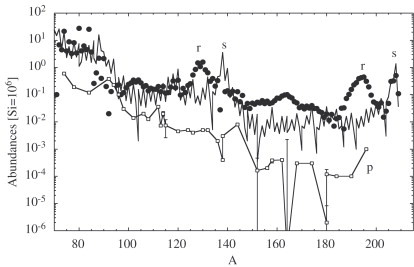
\includegraphics[width=0.5\textwidth]{other_data/arnould_plots/fig1_p100_arnould07_process_decomp.jpg}
  \includegraphics[width=0.5\textwidth]{other_data/arnould_plots/fig4_p220_landholt93_sncp.png}
  \includegraphics[width=0.5\textwidth]{other_data/arnould_plots/fig5_p209_landholt93_rncp.png}
  \includegraphics[width=0.5\textwidth]{other_data/arnould_plots/fig7_p211_landolt93_sos.png}
\end{figure}

In this project, the r-process is of most interest, since the abundance of \re{187} is solely determined by r-process events and the s-process sites are less debated.
\comment{\\discuss possible sites}

\subsection{Stellar enhancement factor} \label{sec:sef}
The \betadecay of a given nuclei in a given energy state is determined by it's halflife (or decay-constant).
This means that a nuclide heated to an excited energy state can have a vastly different halflife than  it's ground state.
This is true for re{187}, among other radioactive nuclei.
These excited stages have greatly reduced lifespans (see section \ref{sec:betadecay} for more details).
In neutral gas in the interstellar medium the temperatures and densitites are not high enough to excited nuclear states, but stellar environments is another story.
If significant populations of \re{187} reach excited nuclear states, halflife of \re{187} will significantly reduce (meaning the decay-constant will increase).
In order to estimate how such environments affect the decay-constant, an \textit{stellar enhancement factor}, SEF, is considered\mycite{shizuma05}. Where $\lambda_{\scriptscriptstyle \beta}^{\scriptscriptstyle \textrm{eff}} = \textrm{SEF}\times\lambda_{\scriptscriptstyle \beta}$ is the effective \betadecay-constant and $\lambda_{\scriptscriptstyle \beta}$ is the \betadecay-constant for the ground state.
In \mycite{shizuma05} a stellar enhancement factor of $\textrm{SEF}=1.2$ is adopted.

\subsection{Nuclear figures}

\begin{figure}
  \begin{minipage}{0.49\textwidth}
    %use \paperheight as fig-height
%\begin{figure}
  \centering
  \includegraphics[width=\linewidth]{img/nuclear_shells.png}
  \caption[Nuclear shells]{
    \label{img:nuclear-shells}
    Energy states of the nuclear orbitals/shells. This shows how the energy-states group together to form clusters of energy-states separeted by so-called magic numbers.\\
    The energy states are grouped together by their principle quantum number $n$, with their orbital splitting $l$ shown in the left column. As can be seen, each orbital term greater then zero (s=0, p=1, ...) are split into two sub-levels determined by their spin-orbit terms in the second column from the left. The third column represent the number of nucleons possible per level, and the far right column indicate magic numbers\mycite{basdevant2005}{ch.2.4}.\\
    Image credit: Bakken at English Wikipedia [CC BY-SA 3.0], from Wikimedia Commons
  }
%\end{figure}

  \end{minipage}
  \begin{minipage}{0.49\textwidth}
    %Draw atomic structure with nucleus and electrons in simple Bohr-model form
\newlength\elrad
\newlength\prorad
\newlength\orbit
\setlength\elrad{0.5mm}
\setlength\prorad{2\elrad}
\setlength\orbit{1cm}

\newcommand\particle[4]{\draw[fill=#4] (#1,#2) circle [radius=#3]}
\newcommand\electron[2]{\particle{#1}{#2}{\elrad}{blue}}
\newcommand\neutron[2]{\particle{#1}{#2}{\prorad}{gray}}
\newcommand\proton[2]{\particle{#1}{#2}{\prorad}{red}}

\centering
\begin{tikzpicture}
    %nucleus
    \proton{-\prorad}{0};
    \proton{\prorad}{2\prorad};
    \proton{\prorad}{-2\prorad};
    \proton{-2\prorad}{\prorad};
    \proton{-2\prorad}{-\prorad};
    \proton{3\prorad}{0};
    \neutron{\prorad}{0};
    \neutron{-\prorad}{2\prorad};
    \neutron{-\prorad}{-2\prorad};
    \neutron{2\prorad}{\prorad};
    \neutron{2\prorad}{-\prorad};
    \neutron{-3\prorad}{0};
    %inner orbit
    \draw (0,0) circle [radius=\orbit];
    \electron{0}{\orbit};
    \electron{0}{-\orbit};
    %outer orbit
    \setlength\orbit{2\orbit}
    \draw (0,0) circle [radius=\orbit];
    \electron{0}{\orbit};
    \electron{0}{-\orbit};
    \electron{\orbit}{0};
    \electron{-\orbit}{0};
\end{tikzpicture}
\caption[Atomic structure]{\label{tikz:atomic-structure}
    Figurative representation of a \isotope{C}{6}{12}-atom with six protons, neutrons, and electrons. The protons (red) and neutrons (gray) occupy the nucleus in the center, while the electrons (blue) orbit around them. According to quantum physics the electrons do not rotate around the nucleus in spherical orbits, but occupy orbitals/energy states around the nucleus as probability distributions. Real and relative sizes do not apply.
    }
  

    %\begin{figure} 
\centering 
\includegraphics[width=\linewidth]{img/binding_energy_curve.png}
\caption[Binding energy per nucleon]{\label{img:binding-energy-curve}
The binding energy per nucleon in the nucleus for isotopes up to \isotope{U}{92}{238}. The peak at \isotope{Fe}{26}{56} means that the nucleons are most tightly bound, and have the least amount of potential energy. \\
Image Credit: Wikipedia Commons
}
%\end{figure}

  \end{minipage}
\end{figure}

\FloatBarrier

\section{Stellar evolution}
\comment{This section is summarized from \mycitetwo{carroll2007}{ch.12,13,15}}

%use textwidth as width of image
\begin{figure}
  \centering
  \includegraphics[width=\figwidth]{img/molecular_cloud.jpg}
  \caption[Hidden secrets of a massive star-formation region]{
    \label{img:molecular-cloud}
    ``Hidden secrets of a massive star-formation region'' by the Herschel telescope and ESA.
    A giant molecular cloud producing stars when local overdensities in the gas collapses. \\
    Image credit: ESA/Herschel/PACS, SPIRE/Hi-GAL Project. Acknowledgement: UNIMAP / L. Piazzo, La Sapienza – Università di Roma; E. Schisano / G. Li Causi, IAPS/INAF, Italy
  }
\end{figure}


\usetikzlibrary{arrows, positioning, automata}

\newlength{\circleheight}
\setlength{\circleheight}{1.5cm}
\newlength{\circlewidth}
\setlength{\circlewidth}{3.4cm}
\newlength{\horseplength}
\setlength{\horseplength}{8cm}
\newlength{\verseplength}
\setlength{\verseplength}{6cm}

\newcommand{\initialgastext}{\centering \textbf{Interstellar gas} \\ Characterized by initial mass function of stars that will form}
\newcommand{\starformationtext}{\centering \textbf{Star formation} \\ Collapse of initial gas into stars \\ Characterized by the star formation rate}
\newcommand{\stardeathtext}{\centering \textbf{Death of stars} \\ Explosive ejection of enriched gas \\ Characterized by isotopic yield tables}
\newcommand{\inflowtext}{\centering \textbf{Inflow} \\ Prestine gas from extragalactic medium}
\newcommand{\outflowtext}{\centering \textbf{Outflow} \\ Enriched gas ejected from intergalactic medium}

\centering
\begin{tikzpicture}[bubble/.style={circle, draw}, flow/.style={rounded corners, draw}]
  %Make nodes with circles of text
  \draw (0.5\horseplength,\verseplength) node[bubble] (A) {\parbox{\circlewidth}{\initialgastext}};
  \draw (0,0) node[bubble] (B) {\parbox{\circlewidth}{\starformationtext}};
  \draw (-0.5\horseplength,\verseplength) node[bubble] (C) {\parbox{\circlewidth}{\stardeathtext}};
  \draw (0.5\horseplength, 2\verseplength) node[flow] (D) {\parbox{\circlewidth}{\inflowtext}};
  \draw (-0.5\horseplength, 2\verseplength) node[flow] (E) {\parbox{\circlewidth}{\outflowtext}};

  %curved arrows between bubbles
  \path (A) edge[bend left, ->, ultra thick] (B);
  \path (B) edge[bend left, ->, ultra thick] (C);
  \path (C) edge[bend left, ->, ultra thick] (A);
  \path (D) edge[->, ultra thick] (A);
  \path (C) edge[->, ultra thick] (E);
\end{tikzpicture}
\caption[Stellar enrichment diagram]{\label{tikz:stellar-enrichment}
  Diagram depicting recycling of gas in a one-zone galaxy model.
  Initially the stellar gas is prestine, from big bang nucleosynthesis, just like the inflow from extragalactic gas.
  Stars form from the prestine gas, forming stellar populations from a given star formation rate and initial mass function.
  Stars end their life asymptotic giant branch stars or explosive type 2 supernovae, ejecting enriched material back into the interstellar medium.
  These events leave remnants, like white dwarves, neutron stars and black holes, which can interact with eachother and other stars to produce secondary explosive events.
  Together the explosive events can drive additional outflow of enriched material away from the galaxy, into the extragalactic medium.
  It should noted that this applies to one-zone models of galaxies, which have two sides; the inside and the outside.
  Ignoring all effects from layered structure of galaxies like; circumgalactic medium, disk, bulge, etc.
}

%use \linewidth as fig-width
\begin{figure}
  \centering
  \includegraphics[width=\linewidth]{img/hr_diagram.png}
  \caption[Hertzsprung-Russel diagram]{\label{img:hr-diagram}
    ``The most famous diagram in astronomy is the Hertzsprung-Russell diagram. This diagram is a plot of luminosity (absolute magnitude) against the colour of the stars ranging from the high-temperature blue-white stars on the left side of the diagram to the low temperature red stars on the right side.

This diagram below is a plot of 22000 stars from the Hipparcos Catalogue together with 1000 low-luminosity stars (red and white dwarfs) from the Gliese Catalogue of Nearby Stars. The ordinary hydrogen-burning dwarf stars like the Sun are found in a band running from top-left to bottom-right called the Main Sequence. Giant stars form their own clump on the upper-right side of the diagram. Above them lie the much rarer bright giants and supergiants. At the lower-left is the band of white dwarfs - these are the dead cores of old stars which have no internal energy source and over billions of years slowly cool down towards the bottom-right of the diagram.''
    Image/description credit: Richard Powell [CC BY-SA 2.5] \href{http://www.atlasoftheuniverse.com/hr.html}{atlas of the universe}
  }
\end{figure}

\begin{figure}
  \centering
  \includegraphics[width=\textwidth]{img/various_initial_mass_functions.png}
  \caption{ \label{fig:various-imf}
    A simplified visualization of some of the common initial mass functions in the literature.
    \mycitetwo{cappellari12}{and references therein}, \mycite{salpeter55}, \mycite{kroupa01}, \mycite{chabrier03}, \mycite{miller79}. \\
    image-credit: By JohannesBuchner [CC BY-SA 4.0 (\url{https://creativecommons.org/licenses/by-sa/4.0})], from Wikimedia Commons
  }
\end{figure}


Regions of space with higher baryon-density then their surroundings are called giant molecular clouds.
These gas clouds are the birth place of stars\mycitetwo{carroll2007}{ch.12}.
Giant molecular clouds can have masses between $10^3$ and $10^7$ \msol, and extend between a few and a few hundred parsecs \mycitetwo{murray11}{tab.1}.
The same 32 giant molecular clouds observed in \mycite{murray11} is also estimated to contribute to on third of current, total star formation in the Milky Way.
Some regions of these giant molecular clouds will have even larger overdensities and gravity dictates that these overdense regions will eventually fall in on themselves.
A star is a sphere of gas with high enough density, and subsequentally high enough temperature, to maintain stable fusion processes in the core.

\noindent
\begin{minipage}{\textwidth}
  How large such a subregion must be to collapse is given by the Jeans criterion.
  The virial theorem states that for a gas in equilibrium the relation between kinetic energy from thermal motion, $E_k$, and potential energy from gravitational collapse, $E_p$, is given by eq.\ref{eq:virial-theorem}.
  When a cloud of gas collapses, this virial-theorem-equilibrium no longer holds and the gravitational potential energy is greater than the thermodynamical kinetic energy.
  This unequilibrium is called the Jeans criterion\mycitetwo{carroll2007}{ch.12}.

  For a spherically symmetric gas, with no rotation, magnetic fields, turbulence or pressure from outside forces the mass of the subregion must exceed the Jeans mass, eq.\ref{eq:jeans-mass}, or the region must cover a smaller volume then covered by the Jeans radius, eq.\ref{eq:jeans-length}.
  Including an external gas pressure, $P_0$, gives the Bonnor-Ebert mass criterion, eq.\ref{eq:bonnor-ebert-mass}\mycitetwo{carroll2007}{ch.12}.
  
  Assuming that any pressure-gradient inside the gas is too small to affect the dynamics and that all the gravitational potential energy released is effectively radiated away, making the gas isothermal, all parts of the gas will collapse to a single point at the same time\footnote{Naturally the gas can't collapse to a singularity, but it will collapse to a radius very small compared to the original radius.}.
  This kind of collapse is called homologous collapse and the free-fall time when all gas reaches the ``singular point'' is given by eq.\ref{eq:ff-time-collapse}\mycitetwo{carroll2007}{ch.12}.

\end{minipage}
%\hfill
\begin{flushright}
\begin{minipage}{0.75\textwidth}
  \begin{equation}
    \label{eq:virial-theorem}
    2 E_k + E_p = 0
  \end{equation}
  \begin{equation}
    \label{eq:jeans-mass}
    M_J = \left(\frac{5kT}{G\mu m_H}\right)^{3/2}\left(\frac{3}{4\pi \rho_0}\right)^{1/2}
  \end{equation}  
  \begin{equation}
    \label{eq:jeans-length}
    R_J = \left(\frac{15kT}{4\pi G\mu m_H\rho_0}\right)^{1/2}
  \end{equation}
  \begin{equation}
    \label{eq:bonnor-ebert-mass}
    M_{\scriptscriptstyle \textrm{BE}} = \frac{c_{\scriptscriptstyle \textrm{BE}}\left(\frac{kT}{\mu m_H}\right)^2}{P_0^{1/2}G^{3/2}}
  \end{equation}
  \begin{equation}
    \label{eq:ff-time-collapse}
    t_{ff} = \left(\frac{3\pi}{32G\rho_0}\right)^{1/2}
  \end{equation}
  Where $k$ and $T$ is the thermal energy, $G$ is the newtonian gravitational constant, $\mu$ and $m_H$ is the average moleular weight, $\rho_0$ is the initial density of the subregion, $c_{\scriptscriptstyle \textrm{BE}}=1.18$ is a dimensionless constant.
  $E_k$, $E_p$, $M_J$, $R_J$, $M_{\scriptscriptstyle \textrm{BE}}$, $t_{ff}$ are kinetic energy, potential energy, Jeans mass criterion, Jeans length criterion, Bonnor-Ebert mass criterion and free-fall time, respectively
  %% \begin{equation}
  %%   \label{eq:}
  %% \end{equation}
  %% \begin{array}{c}
  %% \end{array}
\end{minipage}
\end{flushright}

When temperatures increase, some of the heavier elements will ionize and the free electrons bonds with hydrogen. The $H^-$ ions increase the opacity drastically trapping the heat from gravitational potential energy more efficiently.
When this happens the collapse will be adiabatic instead of isothermal, and temperatures will increase.
When the gas becomes dominantly adiabatic, but still has no stable fusion process in the core the cloud of gas is called a protostar.
Small fusion processes and increased opacity increases the effective surface temperature and luminosity of the gas cloud\mycitetwo{carroll2007}{ch.12}.

Any inhomogeneities in density, and pressure gradient can cause fracturing of the collapsing gas, as can the presence rotation, turbulence, and magnetic fields.
Fracturing means that the subregion is divided into smaller regions where the density might not be big enough or several protostars can be created.
This might also lead to binary systems or systems with several stars.
The entire giant molecular cloud can also be considered a collapsing gas, but fracturing causes several stars to be born as separate entities inside.

When the density and temperature in the core becomes sufficiently high, the protostar will synthesize hydrogen into helium through the pp-chain, or if the star is massive enough the CNO-cycle.
This period of the stars life is the longest and is called the main sequence.
In the Hertzsprung-Russel diagram (see figure \ref{img:hr-diagram}) this extended curve is well documented, and higher mass stars will find themselves higher in the diagram (more mass means more pressure which means more efficient fusion processes).
Throughout the stars life in the main sequence the luminosity and effective temperature will increase steadily as the overall mean molecular weight changes in the entire star.
The location in the Hertzsprung-Russel diagram (luminosity and surface temperature) when the star first starts to burn steadily (when the star is born so to speak) is called the zero-age main sequence\mycitetwo{carroll2007}{ch.12}

The total time it takes for a gascloud to collapse and reach the zero-age main sequence is inversely proportional to it's mass\mycitetwo{carroll2007}{ch.12}.
The total time of a stars lifetime will depend on it's nuclear timescale, which is roughly, inversely proportional to mass cubed for hydrogen burning\mycitetwo{carroll}{ch.13}.
In short massive stars are quickly born and die more quickly, while smaller stars take alot more time. This makes the smaller stars more susceptible to effects from nearby massive stars that ionize or explode while the smaller stars are still forming.
Dispite this, observations show that the mass distribution function of stars massively favor low mass stars.

\comment{(include plot of initial mass distributions here?)}

\subsection{Nuclear fusion processes}
During the main sequence, where hydrogen is burned into helium in the core, higher mass stars will have a much higher central temperature and density. This means that the hydrogen burning core will be dominated by the CNO-cycle, and the star will have a convective layer that develops in the envelope and stretches deep into the star.
Stars with lower mass will have cores dominated by the pp-chain because their central temperature is lower. The energy transport will also be mostly radiative from the core out to the envelope.
Very low mass stars will develop convective layer from the center outwards.
As the stars age, more hydrogen will burn into helium, and the mean molecular weight will increase, steadily increasing the temperature, radius and luminosity of the stars on the main-sequence\mycitetwo{carroll}{ch.13}.
\comment{Add ranges of solar masses to the different types of stars}

When the core of a low-mass star is depleted of hydrogen and filled with helium the pp-chain will stop in the core, but it will continue in a shell around the core due to high temperatures. The hydrogen burning shell around the core will provide more energy and cause the envelope to expand, this causes the luminosity to increase, but surface temperature to decrease.
higher mass stars will contract, and the convective layer disappears steadily as the core runs out of hydrogen fuel. The contraction heats the core and hydrogen shell burning will power the star\mycitetwo{carroll}{ch.13}.

More and more helium is accreted onto the inert, isothermal helium core, which will collapse when it reaches the chandrasekhar limit.
The collapse of the core causes heating, which inflates the envelope.
Inflating the envelope causes the surface temperature to decrease, this is called the sub giant branch.
The inflated envelope stabilizes and becomes convective from the large temperature gradient.
The effective energy transport causes the luminosity to increase, and the star moves into the red giant tip.
This leads to the first dredge-up where material from outside the core can be mixed into the upper envelope.
The collapsed core can now start fusing helium into carbon and oxygen through the triple alpha process.
The core will then expand, cooling the hydrogen shell and decrease the overall luminosity of the star. Stars with lower masses will develop a electron degenerate core which will cause the core helium flash once the helium is ``ignited'' nearly simountaneously\mycitetwo{carroll}{ch.13}.

The envelope will contract following the expansion of the helium burning core, causing the effective surface temperature to rise. When stable radius, helium burning core and hydrogen burning shell is reached the star will have settled onto the horizontal branch. This is the main sequence equivalent of helium burning stars. As the helium is exhausted in the core, the core will start to contract, expanding the envelope, and the effective surface temperature will decrease toward the redder side of the horizontal branch\mycitetwo{carroll}{ch.13}.

When the heliumn has been expended in the core, it leaves an inert core of carbon and oxygen with a helium burning shell around it.
The helium burning shell will dominate over the hydrogen burning shell lying on top of it and the increased temperature will cause the hydrogen burning shell to expand.
The decreased density of the hydrogen burning shell lowers nuclear reaction rates.
When the helium burning shell exhausts all it's fuel the envelope will expand and become convective, the ensuing mix of material, from the bottom envelope (helium burning shell) to top envelope is called the second dredge-up.
The convective energy transport is more effective, increasing the luminosity of the star.
In the Hertzsprung-Russel diagram, this moves the star up into the asymptotic giant branch.
At this point, the hydrogen burning shell will dominate the energy production of the star once again.
\comment{order of magnitude estimates}
The ``ash'' from the hydrogen burning shell (the top shell) will ``rain'' down onto the inert helium burning shell (bottom shell).
When the temperature is high enough and the bottom shell has enough material, the bottom shell of helium will ignite.
Due to the isothermal layer of the helium shell, triple alpha burning will commence in the entire shell simountaneously, in an explosive fashion.
This explosion, called the helium shell flash, is less explosive the the helium core flash, but might eject more material because it is closer to the surface.
When the helium has been exhausted once again, the shell compresses and the entire process repeats. The repetition of helium flashes is called the third dredge-up, mixing material from the hydrogen and helium shells into the upper envelope\mycitetwo{carroll}{ch.13}.

During the asymptotic giant branch stars loose alot of their material by ejection into the interstellar medium. e.g. from helium flashes, pulsations of the envelope, high luminosity, low surface gravity, high radiation pressure.
The combination of effects is not surely determined, but simulations and observations show that the mass-loss must be great during this stage\comment{ref to sims/obs paper}.

After the helium-flashes have subsided, the envelope has been ejected, and the shell-burning have stopped, the star remains as a hot inert core of carbon and oxygen (with some hydrogen and helium surrounding it). This remnant is called a white dwarf.
This white dwarf will continue to glow until it has radiated away all it's thermal energy\mycitetwo{carroll}{ch.13}.

\subsection{Evolution of massive stars}
While less massive stars $M \lesssim 8 \msol$ become white dwarves, stars with mass $M \gtrsim 8 \msol$ evolve a bit differently.
They have no helium flashes.
Their high mass means that the central density, pressure, and temperature will be higher.
The hydrogen burning core will fill up with helium, and when sufficient mass has been reached, the helium will start to fuse into carbon and oxygen through the triple alpha process and hydrogen will burn in a shell around it.
The carbon in the core will then continue to fuse with more helium into oxygen and neon, with some sodium and magnesium produced.
The oxygen in the core will eventually start to fuse into silicon, and the silicon will eventually start to fuse into sulfur, argon and iron.
In this high temperature and high density environment, this process will not be straight forward, many different carbon isotopes will fuse with other particles into many different heavier isotopes. The details above outlines the general trend.
Assuming that there is an equilibrium of nuclear reactions, the stellar interior will resemble an onion-like shell structure with the heaviest elements deepest in the star\mycitetwo{carroll}{ch.15}.

Fusion processes cannot produce excess energy for elements heavier than iron, although trace amounts of heavier elements can be created from the excess thermal energy.
In the centre of the core, the free electrons can merge with the free protons to create neutrons and release neutrinos
\comment{add nuclear reactions}
The sudden loss of electrons causes the electron degeneracy to drop suddenly and the centre of the core will collapse supersonically until the density is roughly 3 times the nucleon density.
At this point the centre of the core, consisting of mostly neutrons will experience a repulsive effect of the strong nuclear force.
This is equivalent to a Pauli exclusion principle of neutrons.
The repulsive force causes the core to stiffen and rebound. The shock from the rebounding core meets the falling core on top, causing a shockwave that travels outward from the inner core.

Simulations suggest that the shockwave released will be absorbed by the surrounding layers.
The stalled shockwave leaves a shell of high density behind.
This shell is dense enough to absorb a significant amount of the neutrinos released during collapse.
If a small amount of the neutrino energy is transferred to the stalled shockwave it will restart and eject the surrounding layers into the interstellar medium.
The travelling shockwave can be observed as a type Ib, Ic, or II supernova, also called a core collapse supernova.
The remnant of such an event will be a neutron star or (if the mass is great enough to overcome the repulsive force of the strong nuclear force) a black hole\mycitetwo{carroll}{ch.15}.
\comment{Mass limits of black hole/neutron star, both core and initial mass limits}

\subsection{Type 1a supernova}
Star systems can be both single and binary, a study by \mycite{lada06} estimates that 1/3 of all star systems are binary.
``When a white dwarf (WD) composed of carbon and oxygen accreting mass from a companion star in
a binary system approaches the Chandrasekhar mass [$M_{Ch} \simeq 1.38$ solar masses (\msol)], high temperature
causes the ignition of explosive nuclear burning reactions that process stellar material and produce energy.
The star explodes leaving no remnant, producing a Type Ia supernova (SNIa) (K. Nomoto, F.-K. Thielemann, K. Yokoi, ApJ 286, 644 (1984)).''\mycite{mazzali07}

In the thermonuclear explosion iron peak elements (mostly Ni and Fe isotopes and below) are synthesized and ejected into the interstellar medium.
During accretion, helium and hydrogen burning layers develop and helium flashes occur.
These flashes can cause major mixing of hydrogen into the carbon-layers which again can cause neutron-producing reactions in greater numbers.
Neutron capture processes can occur on the surface of type 1a supernovae if the produced neutron densities are high enough (\mycite{nomoto84}).
The isotope distributions also seemed to fill in some missing yields from type II supernovae.

Typical type 1a supernovae are heated from the deacy of \isotope{56}{28}{Ni} and will eject $\simeq 1.4 \msol$ of material at a ejecta velocity of $\simeq10 Mm s^{-1} \simeq 0.03c$ (\mycite{tanaka16}).

\subsection{Neutron star mergers}
The idea of mergers of compact objects (either neutron stars or black holes) by emission of gravitational waves have been around for a long time. Since these events are rich in neutrons, they have been suggested as a potential site for r-process nucleosynthesis
(\comment{ref BBFH? ref something}).
This makes makes neutron stars particularly intersesting for the problem in this thesis \comment{rewrite?}
The general concept is build on two compact objects orbiting eachother, interacting with the spatial curvature and creating ripples.
These ripples maifest as waves in the fabric of space-time and carry gravitational energy away.
The two objects move closer as a result of the energy-loss, and increases the orbital velocity accordingly (\mycite{tanaka16}).
These gravitational waves distort space itself and can be detected by large laser interferometers that detect spatial disturbances smaller then the width of a nucleus (\mycite{abott16}).

The material ejected from a binary neutron star merger, or a kilonova, is heated from the decay of r-process elements.
The mass and velocity of the material is debated,
but estimates are around $v=30-60 Mms^{-1} = 0.1-0.2c \quad m \simeq 0.01 \msol$ (\mycite{tanaka16}).

During a neutron star merger, the two stars move closer to eachother over time from gravitational radiation. When they are close enough to eachother they will disrupt each others surface, and surround the merging bodies in a cloud of neutron heavy material that is ejected into the interstellar medium.
The forces that pull apart the neutron stars surface is only gravitational pull and centripetal force.
As the main bodies merge, a shock drives ejection of material that will bombard the surrounding cloud.
As the envelope expands from the colliding stars, the density of neutronmatter will drop until extremely neutron-heavy nuclei will form, like droplets from steam.
These nuclei are unstable and will \betadecay to more stable isobars.
These heavy nuclei will act as seeds for the neutronrich shockwave emitting from the collision.
\comment{find proper ref on where seeds come from}
The stream of very dense, high-velocity neutrons onto seed of heavy nuclei is the perfect recipe for r-process nucleosynthesis\mycite{tanaka16}.

\subsection{Debate over site of r-process nucleosynthesis}
\comment{write two sentences of the site-debated with ref. refer to this section in thesis}


\section{The \re{187}-\os{187} chronometer}
In this work, \textit{cosmochronology} refers to dating astrophysical events based, more specifically the age of nucleosynthesis.
A \textit{chronometer} is a pair of radioactive nuclei, with an appropriate halflife which allows us to do exactly that.
As mentioned in section \comment{section nuclear physics with betadecay \ref{sec:betadecay}?}, \re{187} \betadecay{s} to \os{187} with a halflife of 41.6 Gyr (\mycite{snelling15}).
This halflife is appropriate for dating Galactic ages, which occur on the scale of universal ages (The age of the universe, from the Planck collaboration is measured to 13.8 Gyrs \mycite{planck15}).
Because of this, \mycite{clayton64} suggest the \re{187}-\os{187} nuclei as Galactic chronometer, also called a cosmic clock.

\comment{insert tikz chart of nuclides here \\}
From section \comment{nuclear-physics r-process and s-process} it is clear that synthesis of heavy nuclei can be divided into two processes, rapid and slow neutron capture (ignoring proton capture).
Figure \comment{tikz chart of nuclides} show the s-process path and the r-process path in the region around the \re{187}-\os{187}-pair.

\os{187} and \os{187} can only be reached by the s-process, because the r-process material will \betadecay to \re{187} and \w{186} where the halflife is comparable to the age of the universe. Simontaneously, neglecting the \w{184} branching points, the s-process cannot reach \re{187} (\mycite{clayton64}).

This means that \re{187} is synthesized through the r-process and \os{187} is synthesized through the s-process from \os{186} and cosmoradiogenic \betadecay from \re{187}.
By assuming a rate of events producing r-process elements, starting from the age of nucleosynthesis, the amount of cosmoradiogenic \os{187} compared to \re{187} in the interstellar medium Galaxy is calculatable.
This ratio is assumed to be representative of the interstellar medium near the \sos during it's formation.
The same ratio can be found at the formation of the \sos from meteorites today. These meteorites condensed from the dust and gas in the early epoch of the \sos and have remained pure since then until they impacted the earth.

In his model for cosmochronology of Re-Os, \mycite{clayton64} assumes a exponential decay of the rate of r-process events $A(t) = e^{-\Lambda t}$, where an infinite decay constant ($\Lambda\rightarrow\infty$) leads to a ``sudden synthesis'' model and a zero decay constant ($\Lambda\rightarrow 0$) leads to a ``uniform synthesis'' model.
A detailed calculation following these models are presented in appendx \ref{sec:calc-cosmo-chronology}.


\iffalse

\comment{include chart of nuclide section}
%% \begin{figure}
%%   %include tikz if not already done

%define functions for squares
\newcommand{\drawsquare}[3]{ %arguments: x0, y0, width/2
  \draw (#1-#3, #2-#3) -- (#1-#3, #2+#3)
  -- (#1+#3, #2+#3) -- (#1+#3, #2-#3)
  -- (#1-#3, #2-#3);
}
\newcommand\drawnuclide[4]{ %arguments: square-x0, square-y0, square-width/2, nuclide
  \drawsquare{#1}{#2}{#3};
  \draw (#1,#2) node {#4}
}
\newcommand\fillrectangle[3]{ %arguments: x0, y0, width/2
  \fill[color=lightgray,opacity=0.2, pattern=north west lines, pattern color=darkgray]
  (#1-#3, #2-#3) rectangle (#1+#3, #2+#3)
}

\newlength{\halfwidthnuclides}
\newlength{\distancenuclides}
\newlength{\offset}
\setlength{\halfwidthnuclides}{5mm}
\setlength{\distancenuclides}{3\halfwidthnuclides}
\setlength{\offset}{0.5\halfwidthnuclides}

\usetikzlibrary{patterns}

%\begin{figure}
\centering
\begin{tikzpicture}
  %test in the middle
  %\draw (0,0) node {${}^{A+1}_{Z}$X};
  %\tikzsquare{0}{0}{\halfwidthnuclides}
  %Os-row on top of test
  \iffalse %old version
  \draw (-\distancenuclides,\distancenuclides) node {${}^{186}_{76}$Os};
  \tikzsquare{-\distancenuclides}{\distancenuclides}{\halfwidthnuclides}
  \draw (0,\distancenuclides) node {${}^{187}_{76}$Os};
  \tikzsquare{0}{\distancenuclides}{\halfwidthnuclides}
  \draw (\distancenuclides,\distancenuclides) node {${}^{188}_{76}$Os};
  \tikzsquare{\distancenuclides}{\distancenuclides}{\halfwidthnuclides}
  %stable Re-isotopes
  \draw (-\distancenuclides,0) node {${}^{185}_{75}$Re};
  \tikzsquare{-\distancenuclides}{0}{\halfwidthnuclides}
  \draw (\distancenuclides,0) node {${}^{187}_{75}$Re};
  \tikzsquare{\distancenuclides}{0}{\halfwidthnuclides}
  %W island of stability
  \draw (\distancenuclides,-\distancenuclides) node {${}^{186}_{74}$W};
  \tikzsquare{\distancenuclides}{-\distancenuclides}{\halfwidthnuclides}
  %shaded region of stability
  \fill[color=lightgray,opacity=0.1, pattern=north west lines, pattern color=darkgray]
  (-0.5\distancenuclides,-0.5\distancenuclides)
  rectangle (-1.5\distancenuclides,1.5\distancenuclides)
  rectangle (1.5\distancenuclides,0.5\distancenuclides)
  rectangle (0.5\distancenuclides,-1.5\distancenuclides);
  \fi

  %draw stable nuclei from clayton64 fig.1.
  %row1 - Os-184, blank, Os-186, Os-187, Os-188, Os-189
  \drawnuclide{-3\distancenuclides}{\distancenuclides}{\halfwidthnuclides}{\os{184}};
  \drawsquare{-2\distancenuclides}{\distancenuclides}{\halfwidthnuclides};
  \drawnuclide{-\distancenuclides}{\distancenuclides}{\halfwidthnuclides}{\os{186}};
  \drawnuclide{0}{\distancenuclides}{\halfwidthnuclides}{\os{187}};
  \drawnuclide{\distancenuclides}{\distancenuclides}{\halfwidthnuclides}{\os{188}};
  \drawnuclide{2\distancenuclides}{\distancenuclides}{\halfwidthnuclides}{\os{189}};
  %row2 - blank, blank, Re-185, blank, Re-187, blank
  \drawsquare{-3\distancenuclides}{0}{\halfwidthnuclides};
  \drawsquare{-2\distancenuclides}{0}{\halfwidthnuclides};
  \drawnuclide{-\distancenuclides}{0}{\halfwidthnuclides}{\re{185}};
  \drawsquare{0}{0}{\halfwidthnuclides};
  \drawnuclide{\distancenuclides}{0}{\halfwidthnuclides}{\re{187}};
  \drawsquare{2\distancenuclides}{0}{\halfwidthnuclides};
  %row3 - W-182, W-183, W-184, blank, W-186, blank
  \drawnuclide{-3\distancenuclides}{-\distancenuclides}{\halfwidthnuclides}{\w{182}};
  \drawnuclide{-2\distancenuclides}{-\distancenuclides}{\halfwidthnuclides}{\w{183}};
  \drawnuclide{-\distancenuclides}{-\distancenuclides}{\halfwidthnuclides}{\w{184}};
  \drawsquare{0}{-\distancenuclides}{\halfwidthnuclides};
  \drawnuclide{\distancenuclides}{-\distancenuclides}{\halfwidthnuclides}{\w{186}};
  \drawsquare{2\distancenuclides}{-\distancenuclides}{\halfwidthnuclides};
  %row4 - Ta-181, blank, blank, blank, blank, blank
  \drawnuclide{-3\distancenuclides}{-2\distancenuclides}{\halfwidthnuclides}{${}^{181}_{73}$Ti};
  \drawsquare{-2\distancenuclides}{-2\distancenuclides}{\halfwidthnuclides};
  \drawsquare{-\distancenuclides}{-2\distancenuclides}{\halfwidthnuclides};
  \drawsquare{0}{-2\distancenuclides}{\halfwidthnuclides};
  \drawsquare{\distancenuclides}{-2\distancenuclides}{\halfwidthnuclides};
  \drawsquare{2\distancenuclides}{-2\distancenuclides}{\halfwidthnuclides};

  %shaded region of stability
  \fillrectangle{-3\distancenuclides}{-2\distancenuclides}{0.5\distancenuclides}; %Ta-181
  \fillrectangle{-3\distancenuclides}{-\distancenuclides}{0.5\distancenuclides}; %W-182
  \fillrectangle{-2\distancenuclides}{-\distancenuclides}{0.5\distancenuclides}; %W-183
  \fillrectangle{-\distancenuclides}{-\distancenuclides}{0.5\distancenuclides}; %W-184
  \fillrectangle{-\distancenuclides}{0}{0.5\distancenuclides}; %Re-185
  \fillrectangle{-\distancenuclides}{\distancenuclides}{0.5\distancenuclides}; %Os-186
  \fillrectangle{0}{\distancenuclides}{0.5\distancenuclides}; %Os-187
  \fillrectangle{\distancenuclides}{\distancenuclides}{0.5\distancenuclides}; %Os-188
  \fillrectangle{2\distancenuclides}{\distancenuclides}{0.5\distancenuclides}; %Os-189
  %\fillrectangle{\distancenuclides}{0}{0.5\distancenuclides}; %Re-187
  %\fillrectangle{\distancenuclides}{-\distancenuclides}{0.5\distancenuclides}; %W-186

  %draw s-process path
  \draw [ultra thick, ->, blue] (-2\distancenuclides-\offset,-3\distancenuclides-\offset)
  -- (-3\distancenuclides+\offset,-2\distancenuclides-\offset) -- (-2\distancenuclides-\offset,-2\distancenuclides-\offset)
  -- (-3\distancenuclides+\offset,-\distancenuclides-\offset) -- (0-\offset,-\distancenuclides-\offset)
  -- (-\distancenuclides+\offset,0-\offset) -- (0-\offset,0-\offset)
  -- (-\distancenuclides+\offset,\distancenuclides-\offset) -- (3\distancenuclides-\offset,\distancenuclides-\offset);
  %draw s-process branching point
  \draw [ultra thick, dashed, blue] (-\distancenuclides+\offset,-\distancenuclides-\offset)
  -- (2\distancenuclides-\offset,-\distancenuclides-\offset) -- (\distancenuclides+\offset,0-\offset)
  -- (2\distancenuclides-\offset,0-\offset) -- (\distancenuclides+\offset,\distancenuclides-\offset);
  \draw [ultra thick, dashed, blue] (-\distancenuclides+\offset,0-\offset)
  -- (2\distancenuclides-\offset,0-\offset);

  %draw r-process paths
  \draw [ultra thick, dotted, ->, red] (0+\offset,-3\distancenuclides-\offset)
  -- (-2\distancenuclides+\offset,-\distancenuclides-\offset);
  \draw [ultra thick, dotted, ->, red] (\distancenuclides+\offset,-3\distancenuclides-\offset)
  -- (-\distancenuclides+\offset,-\distancenuclides-\offset);
  \draw [ultra thick, dotted, ->, red] (1.5\distancenuclides+\offset,-2.5\distancenuclides-\offset)
  -- (-\distancenuclides+\offset,0-\offset);
  \draw [ultra thick, dotted, ->, red] (3\distancenuclides+\offset,-3\distancenuclides-\offset)
  -- (\distancenuclides+\offset,-\distancenuclides-\offset);
  \draw [ultra thick, dotted, ->, red] (3\distancenuclides+\offset,-2\distancenuclides-\offset)
  -- (\distancenuclides+\offset,0-\offset);
  \draw [ultra thick, dotted, ->, red] (3\distancenuclides+\offset,-\distancenuclides-\offset)
  -- (\distancenuclides+\offset,\distancenuclides-\offset);

  %add text
  \addtolength\offset{1.8\offset}
  \draw (-3\distancenuclides, -3\distancenuclides) node[thick, draw, blue] {s-process};
  \draw (2\distancenuclides, -3\distancenuclides) node[thick, draw, red] {r-process};
  \draw (0,0+\offset) node[draw=magenta, magenta, rounded corners] {${\scriptscriptstyle T_{\beta}=89hr}$}; %halflife of Re-186
  \draw (0,-\distancenuclides+\offset) node[draw=magenta, magenta, rounded corners] {${\scriptscriptstyle T_{\beta}=76d}$}; %halflife of W-185
  \draw (\distancenuclides,0+\offset) node[draw=magenta, magenta, rounded corners] {${\scriptscriptstyle T_{\beta}=41.6Gyr}$}; %halflife of Re-187
  \addtolength\offset{-1.8\offset}
\end{tikzpicture}
\caption[Chart of nuclides from \mycitetwo{clayton64}{fig.1} around A=187]{\label{tikz:nuclide-chart}
  Chart of nuclides around massnumber 187, adopted from \mycitetwo{clayton64}{fig.1}.
  The stable nuclei are denoted with their chemical symbols.
  The path of the s-process follows the valley of stability (shaded region), and is drawn as a blue solid line.
  Neutrons are absorbed during the s-process until and unstable isotope is reached, the unstable nuclide then \betadecay{s} to the higher isobars\footnote{the highest stable isobar means the nuclei with the same amount of nucleons and the highest amount of protons}.
  R-process nuclei are already very neutron-rich, and \betadecay{s} to the highest stable isobar.
  The path of the r-process is shown as red dotted lines.
  \w{185}, and also \re{186}, are potential branching points (), and can cause branched s-proces paths that are shown as blue dashed lines.
  The half-lifes of these potential branching point nuclei, as well as the half-life of \re{187}, are written in magenta over the nuclei.
}

%% \end{figure}


From the chart on can see the usual path for slow neutron capture along the valley of stability.
This is the main contribution to \os{187}. In a standard s-process analysis, \w{185} and \re{186} are unstable, and will decay before they can capture neutrons. The s-process path will never synthesize \re{187}. However if the neutron capture rate is comparable to the \betadecay rates of those nuclides a branching point can occur. A branching point is a point where the synthesizing path of the s-process split due to competing nuclear reactions. In this case a significant fraction of the s-process path can go through \re{186} to \re{187} or through \w{185} to \w{186} (which is stable) and onwards to \re{187}. Apart from these effects \re{187} is shielded from s-process contribution.

The rapid neutron capture maintains very high neutron numbers until the neutron source ``shuts off'', at that point the isotopes \betadecay to the valley of stability. Given the long \halflife of \re{187} it can be considered stable, so the \os{187} isotope is shielded from r-process contribution because almost all \betadecay on the 187-isobar will stop at \re{187}.

Since \re{187} is radioactive with a halflife of \comment{add here} some \re{187} in the interstellar or stellar medium will decay to \os{187}. This amount is called the cosmoradiogenic \os{187}. The fraction between cosmoradiogenic \os{187} and current \re{187} is given by the exponential decay-function (assuming ofcourse that the nuclear decay rate is constant for all time, including stellar environments), meaning the time of nucleosynthesis can be calculated from the observed fraction of daughter-parent nuclei.

Clayton attempts to calculate the fraction of cosmoradiogenic osmium and the age of nucleosynthesis from these principles\mycite{clayton64}.
A brief summary follows:

The abundance of \os{186} is due to s-process only, and the abundance of \os{187} is due to s-process (from \os{186}) and cosmo radiogenic enrichment from \re{187} beta-decay.
The s-process contribution from \os{186} is given by the \os{186} abundance and the ratio between the cross-section of the isotopes. It is shown from nebular Samarium that the two s-only isotopes have nearly identical cross-section times abundance. Extrapolating this to other s-process isotopes, the result is:
(denoting abundance of isotope by their chemical name instead of N for simplicity)
\begin{equation}
  \bar{\sigma}_{\os{186}}{\os{186}} = \bar{\sigma}_{\os{187}}{\os{186}_S}
  \quad \rightarrow \quad
  {\os{186}_S} = \frac{\bar{\sigma}_{\os{186}}}{\bar{\sigma}_{\os{187}}}{\os{186}}
\end{equation}
$\bar{\sigma}$ are the neutron-capture cross-sections averaged over the appropriate thermal velocity distributions.
The cosmoradiogenic component of \os{187} is therefor the remaining part.
\begin{equation}
  \os{187}_c = \os{187} - \os{187}_s = \os{187} - \frac{\bar{\sigma}_{\os{186}}}{\bar{\sigma}_{\os{187}}}{\os{186}}
\end{equation}
Rewriting equation to relative units.
\begin{equation}
  \frac{\os{187}_c}{\re{187}} = \frac{\os{187} - \frac{\bar{\sigma}_{\os{186}}}{\bar{\sigma}_{\os{187}}}{\os{186}}}{\re{187}} =
  \frac{
    \left(\frac{\os{187}}{Os}\right) -
    \frac{\bar{\sigma}_{\os{186}}}{\bar{\sigma}_{\os{187}}}
    \left(\frac{\os{186}}{Os}\right)
  }{
    \left(\frac{\re{187}}{Re}\right)
  }
  \left(\frac{Os}{Re}\right)
\end{equation}
Origin of time, t=0, is set to \sos formation. Assuming that r-process events are supernovae and they began occuring at time T before \sos formation(t=0), and the frequency of events decreases exponentially as $f_0e^{\Lambda t}$, where $f_0$ is the initial supernovae freqency.
According to this model, and Clayton, the amount of cosmoradiogenic \os{187} is given by
\begin{equation}
  \frac{\os{187}_c}{\re{187}} = \left[
    \frac{\Lambda-\lambda}{\Lambda}
    e^{\lambda T}
    \frac{1-e^{-\Lambda T}}{1-e^{-(\Lambda-\lambda) T}}
    \right] - 1
\end{equation}
And the two special cases. \\
Sudden synthesis ($\Lambda\rightarrow\infty$)
\begin{equation}
  \frac{\os{187}_c}{\re{187}} = e^{\lambda t} - 1
\end{equation}
Uniform synthesis ($\Lambda\rightarrow 0$)
\begin{equation}
  \frac{\os{187}_c}{\re{187}} = \frac{\lambda T}{1-e^{-\lambda t}} - 1
\end{equation}

\comment{end of direct summary}

In short, by modelling r-process nucleosynthesis and s-process nucleosynthesis, the fraction of \re{187}-\os{187} in the \sos can predict the time of nucleosynthesis from non-cosmological methods.
\comment{\\ What do I mean about the age of nucleosynthesis?}
\fi


%theory II
\chapter{Theory Part II \comment{(need to rename)}}
\comment{Describe analytical models, numerical models (omega), simulations (eris) and that I compare the two latter}
\comment{Results from omega can be compared to hydrodynamical simulations like eris. Which are much more detialed and precise, but also more computationally expensive.}
\setlength{\figwidth}{0.8\linewidth}
\section{The \omegamodel\ model}
\label{sec:omega}
\omegamodel\ is a python code developed by Benoit C\^{o}t\'{e} and Christian Ritter\footnote{\url{https://nugrid.github.io/NuPyCEE/}}.
OMEGA stands for 'One-zone Model of the Evolution of Galaxies' and evolves the isotopic content of a galaxy\mycite{cote16a}.
The model is a one-zone model, which means that the entire galaxy is simplified to a single point.
A zero-space-dimensional galaxy model seems unrealistic, but it can be imagined as the mean value for a three-space-dimensional galaxy model.

\begin{figure}
  %Define useful lengths
\newlength{\boxwidth}
\setlength{\boxwidth}{2cm}
\newlength{\boxheight}
\setlength{\boxheight}{1.5cm}
\newlength{\boxdepthx}
\setlength{\boxdepthx}{0.5\boxwidth}
\newlength{\boxdepthy}
\setlength{\boxdepthy}{0.5\boxheight}

%Define useful positions w/short-hand notation
%pos-position, b-bottom, t-top, l-left, r-right, f-front, d-distant
\newcommand\posbfl{(-\boxwidth,-\boxheight)}
\newcommand\posbfr{(\boxwidth,-\boxheight)}
\newcommand\posbdr{(\boxwidth+\boxdepthx,-\boxheight+\boxdepthy)}
\newcommand\posbdl{(-\boxwidth+\boxdepthx,-\boxheight+\boxdepthy)}
\newcommand\postfl{(-\boxwidth,\boxheight)}
\newcommand\postfr{(\boxwidth,\boxheight)}
\newcommand\postdr{(\boxwidth+\boxdepthx,\boxheight+\boxdepthy)}
\newcommand\postdl{(-\boxwidth+\boxdepthx,\boxheight+\boxdepthy)}

\begin{figure}
  \centering
  \begin{tikzpicture}
    %insert galaxy-image in center
    \node (galaxy) at (0.5\boxdepthx,0.5\boxdepthy) {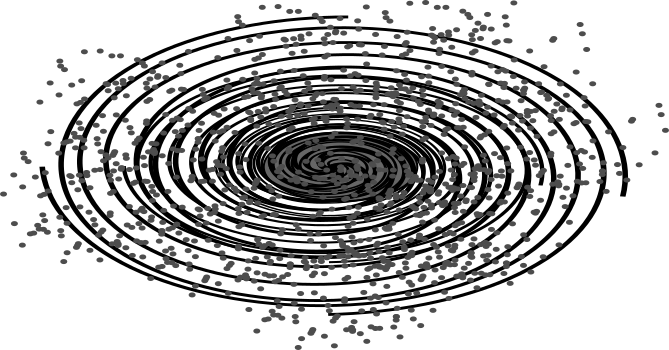
\includegraphics[width=\boxwidth]{galaxy_thumbnail/galaxy.png}};
    %draw bottom plate
    \draw \posbfl -- \posbfr -- \posbdr -- \posbdl -- \posbfl;
    %draw top plate
    \draw \postfl -- \postfr -- \postdr -- \postdl -- \postfl;
    %draw vertical connectors
    \draw \posbfl -- \postfl;
    \draw \posbfr -- \postfr;
    \draw \posbdl -- \postdl;
    \draw \posbdr -- \postdr;
    %add inflow above box
    \draw[thick,->] (0,1.5\boxheight+\boxdepthy) -- (0,1.2\boxheight+\boxdepthy);
    %\draw (-0.5\boxdepthx,2\boxheight) -- (0,2\boxheight-0.5\boxdepthx) -- (0.5\boxdepthx,2\boxheight);
    %\draw (-0.25\boxdepthx,3\boxheight) -- (-0.25\boxdepthx,2\boxheight);
    %\draw (0.25\boxdepthx,3\boxheight) -- (0.25\boxdepthx,2\boxheight);
    \node at (0.6\boxwidth, 1.3\boxheight+\boxdepthy) {\small Primordial gas};
    %add outflow below box
    \draw[thick,->] (0,-1.2\boxheight) -- (0,-1.5\boxheight);
    %\draw (-0.5\boxdepthx,-2\boxheight) -- (0,-2\boxheight-0.5\boxdepthx) -- (0.5\boxdepthx,-2\boxheight);
    %\draw (-0.25\boxdepthx,-1\boxheight) -- (-0.25\boxdepthx,-2\boxheight);
    %\draw (0.25\boxdepthx,-1\boxheight) -- (0.25\boxdepthx,-2\boxheight);
    \node at (0.6\boxwidth, -1.3\boxheight) {\small Enriched gas};
  \end{tikzpicture}
  \caption{\label{tikz:galaxy-iobox}}
\end{figure}

\end{figure}

In this work the \omegamodel\ code will be modified with a wrapper in order to explore various parameters related to nucleosynthesis.

\subsection{Process}
\label{sec:omega-process}
The \omegamodel\ model emulates the chemical evolution of a galaxy starting from the initial primordial gas. A simple stellar population is created by integrating the star formation rate over time.
The star formation rate is calculated either by using a constant star formation rate, the Kennicut-Schmidt law\mycitetwo{fuchs09}{and refernces therein}, or by using an input star formation rate and interpolate over those values.

The stellar populations represent a cluster of stars, with a total mass, initial mass distribution, and initial metallicity distribution.
The initial mass distributions are given as one of the standard distributions, Salpeter, Kroupa, Chabrier, or a power-law, all between some minimum and maximum mass limit (see figure \ref{fig:imf}.
The initial metallicity distribution is the relative mass distribution of isotopes heavier than \isotope{Li}{3}{7}, and the metallicity is the mass fraction of all isotopes heavier than \isotope{Li}{3}{7} combined.
\begin{figure}
  \centering
  \includegraphics[width=\textwidth]{img/various_initial_mass_functions.png}
  \caption{ \label{fig:various-imf}
    A simplified visualization of some of the common initial mass functions in the literature.
    \mycitetwo{cappellari12}{and references therein}, \mycite{salpeter55}, \mycite{kroupa01}, \mycite{chabrier03}, \mycite{miller79}. \\
    image-credit: By JohannesBuchner [CC BY-SA 4.0 (\url{https://creativecommons.org/licenses/by-sa/4.0})], from Wikimedia Commons
  }
\end{figure}


Stellar evolution codes calculate the amount of ejected material, for each isotope, for a star with a given initial metallicity and initial mass. These codes are used to create \textbf{yield tables} for certain kind of stars with different initial mass and metallicity.

In the simple stellar population assumed in the galactic chemical evolution model, these yield tables are used to calculate the chemical composition and mass of ejecta from each group of stars. The ejecta are disspersed back into the interstellar medium (gas of the galaxy model) at delay-times appropriate for each group of stellar mass.
E.g. For a given mass-bin the total mass in stars, number, and age of stars, with initial mass in that bin, are calculated using the total mass of the total stellar mass and mass function chosen. By choosing the yield tables closest in initial mass and initial metallicity the total ejecta composition is calculated and added to the interstellar medium at the age where those stars would have gone supernova.
The material that is not ejected is left as remnants and total mass and number of remnants are also added to the simulation at the time these stars would have gone supernova.

In \omegamodel\ the creation and treatment of simple stellar population is done by another python-program called \texttt{Sygma}.

The \omegamodel\ model is a \textit{one-zone} model, meaning that everything inside the box has been enriched from stellar lifecycles. Everything outside the box is untouched since ``it's creation'', and has the same composition as the material inside the box had to start with.
This composition is called the primordial composition (three parts hydrogen, one part helium and trace amounts of lithium and beryllium), and is derived from the big bang nucleosynthesis (see section\ref{sec:bbn}.
Flow of material can determine the chemical evolution of a galaxy. Enriched material can be ejected from the galaxy by supernova feedback, active galactic nucleus, stellar kick or similar, and non-enriched material can flow into the galaxy.
To describe the chemical evolution of a one-zone model one needs to know the total content of the galaxy (or box) and the distribution. In other words, how much of the total mass is stored as each isotope. Material with the same composition as the box is ejected from the box, and material with another composition falls into the box.

\comment{More on outflow/inflow}

\comment{Insert simple figure here}

\subsection{Uncertainty of parameters}
\comment{uncertainty of parameters and summary of article (cote16a)}

Galaxies consist of many different, widely varying, scales for both spatial and temporal resolution.
The galaxies themselves span hydrodynamical evolution on many kpcs and Gyrs, while their stars and supernovae span scales closer to seconds and meters.
The nuclear processes within stars span nanometer and millisecond timescales, even though stars can last for billion years(with short timescale bursts in between).
Neither analytical/numerical models nor simulations cannot cover all these scales at once, that is when subgrid methods are used. Stellar evolution simulations predict the fate and output from the life of a single star based on sinple input parameters and assumptions of the physical processes that governs the evolution. These solutions are then simplified and applied to more complex galaxy simulations.
Output ejecta from stars are ``looked up in a table'' and applied to the nearby interstellar medium.
All these methods and linked applications introduce some uncertainties and assumptions, both physical and numerical, and these uncertainties are inherited through all methods based on applications of these models. In order to probe how the uncertainties of selected parameters manifest through the resulting galaxy evolution, \mycite{cote16a} presents a simple one-zone, closed-box model of galaxy evolution, called \omegamodel.

%use \figwidth for width of image
\begin{figure}
  \centering
  \includegraphics[width=\figwidth]{img/uncertainty_diagram_cote16a_fig1.png}
  \caption[\mycitetwo{cote16a}{fig.1}]{ \label{img:uncertainty-diagram}
    Qualitative visualization of how uncertainties accumulate in galactic chemical evolution models.
    Experimental data on nuclear reaction rates are uncertain to some degree. The change in rate and uncertainty in stellar conditions are not well known.
    The conditions inside a star of a given mass and metallicity come from 1 dimensional hydrodynamical simulations.
    The combined result from nuclear reactions and hydrodynamical simulations give a stellar models.
    The stellar models are applied to a simple stellar population to account for all the billions of stars in galaxy.
    These stellar models are then applied to a large scale hydrodynamical simulation (like \eris), or a semianalytical galaxy model (like \omegamodel).
    All the steps make assumptions and add uncertainty to the grand total uncertainty that is difficult to map in completeness.

    Diagram is taken from \mycitetwo{cote16a}{fig.1}
  }
\end{figure}


\sygma creates the simplified stellar populations (mass function, total mass, lifetime distribution, initial metallicity).
\omegamodel\ combines several stellar populations to emulate a galaxy evolution.

Stellar yields are tables from stellar evolution simulations.
The tables used in \omegamodel are taken from, among other sources,  NuGrid\footnote{NuGrid collaboration: \href{http://www.astro.keele.ac.uk/nugrid/}{Homepage} \href{https://github.com/nugrid}{Github}} and include AGB stars between 1 and 7 \msol, massive stars between 12 and 25 \msol, all with metallicities at $Z = 0.02, 0.01, 0.006, 0.001, 0.0001$. These tables contain many isotopes between hydrogen and bismuth.

The stellar evolution was calculated with MESA\footnote{MESA is a modular, opensource code to evolve single star systems, and can do so from main sequence to white dwarf stage or core collapse stage. See \href{http://mesa.sourceforge.net}{Homepage} for further information}, post-processing was done with MPPNP \mycite{nugrid08mppnp}, the same nuclear reaction rates were used in all calculations, explosive nucleosynthesis was done with semi-analytical models. Yields are complemeted with SN1a yields from \mycite{sn1aivo13}, \mycite{sn1at03}, \mycite{sn1ai99}, \mycite{sn1at86} and population III yields from \mycite{pop3hw10} (other sources are available from the literature, but these are the focus of the chemical evolution of this thesis. Sources for neutron star mergers will be discussed later).

The probability distribution functions for the input parameters are created from values and uncertainties in the literature.
Methodologically there are, for each input parameter, gathered a list of literature values and uncertainties.
The errors are considered gaussian in nature and distributions are created thereafter,
all the distributions are then averaged to a single distribution.
Then a single gaussian is fitted atop the ``average of gaussians from the literature'',
and the median and standard deviation from
the final fit is used as value and uncertainty for the input parameter in question.

%insert images from cote16a to summarize the parameter-method
\setlength{\subfigwidth}{\linewidth}
\begin{figure}
  \centering
  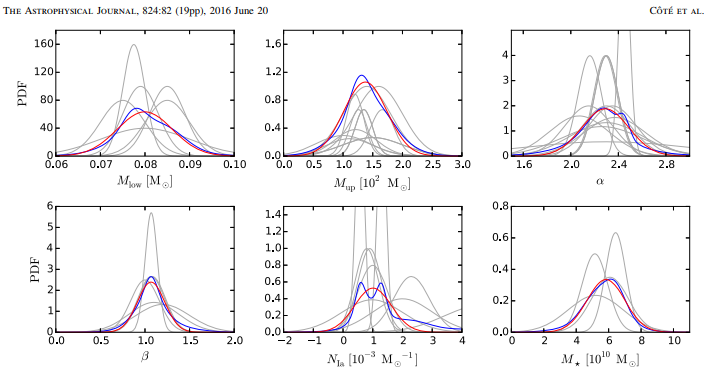
\includegraphics[width=\subfigwidth]{img/parameter_pdfs_cote16a_fig2.png}
  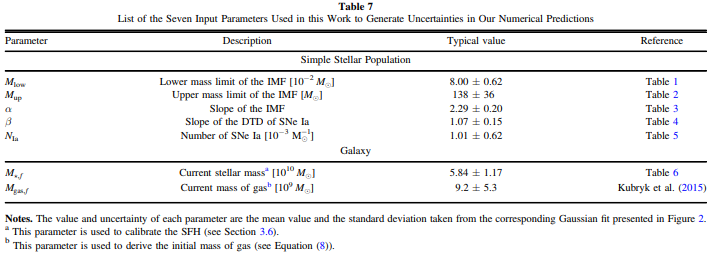
\includegraphics[width=\subfigwidth]{img/parameter_table_cote16a_table7.png}
  \caption{\label{fig:cote16-input-param}
    How the input parameters were determined from multiple sources in the literature. Values and standard deviations averaged to a probaiblity distribution, and then fitted to a single gaussian distribution. Images from \mycitetwo{cote16a}{figure 2 and table 7}.
  }
\end{figure}

\mycite{cote16a} sampled a set calculations, for each parameter in figure \ref{fig:cote16-input-param} a series of 300 calculations were made with a random sampling of the input parameter for the gaussian uncertainty distribution.
A set of 700 calculations were made were all the input parameters were all the input parameters were randomly drawn from their respective gaussian distributions. An additional 300 calculations were made with the final gas-mass and final stellar mass both drawn randomly from their respective gausssian distributions.

Spectroscopic abundance of metals are measured in [X/Y] where X is the metal in question and Y is the reference metal, either plotted against metallicity, [Y/H], or galactic time, Gyr.

The main conclusions are summarized as follows:
\begin{enumerate}
\item{
  The overall uncertainty of spectroscopic metals between 0 and 0.6 dex when plotted against metallicity, but the uncertainty is higher when considered against galactic time.}
\item{
  \begin{itemize}
  \item{Ratio of final mass of gas to final mass of stars affect the uncertianty for early times ([Fe/H] $\lesssim$ -2) since more gas means more hydrogen, while more stars means more iron-production. Since metals are also produced in stars, the ratio does not affect [X/fe] much.}
  \item{Number of type 1a supernovae and their delay time distribution affect the uncertainty of spectroscopic metals at later times([Fe/H] $\gtrsim$ -1.5 $\rightarrow$ t $\gtrsim$ 150Myr), when the delay-time has allowed for type 1a supernovae to occur. Type 1a supernovae add mostly iron to the interstellar medium, while not producing much of metals produced by AGB stars and massive stars. This means that the uncertainty of [X/Fe] will be greatly affected by uncertianties in type 1a supernovae.}
  \item{The high mass slope of the initial mass function, $\alpha$, determines the ratio of massive stars to low-mass stars at all times. Massive stars die quickly and distributed much enriched material into the interstellar medium. Therefor the uncertainty of the slope will always be prevailent in the uncertainty of spectroscopic metals.}
  \item{Uncertainties in the mass ranges of the initial mass function does not affect uncertainties of the spectroscopic abundances much.}
  \end{itemize}
}
\item{
  Uncertainties in the slope of the initial mass function, $\alpha$, and the number of type 1a supernovae affect the uncertainties in the spectroscopic abundances.
  When plotted against metallicity ([Fe/H]) the uncertainty is greatest when the considered metal and the reference metal is not from the same source.
}
\item{
  The characteristics seen from spectroscopic abundance against metallicity is shared regardless of the introduced uncertainties.
  The introduced uncertainties amplify the characterstic shapes, but do not change them. ``Such features are mainly caused by the choice of stellar yields and the type of galaxy considered.''\mycitetwo{cote16a}{p.18}
}
\end{enumerate}

%use \figwidth for width of figure

\begin{figure}
  \centering
  \includegraphics[width=\figwidth]{img/spectroscopic_uncertainties_cote16a_fig6.png}
  \caption[\mycitetwo{cote16a}{fig.6}]{
    \label{img:spectroscopic-uncertainty}
    Spectroscopic abundance of 16 metals relative to iron, considering uncertainties of all parameters (upper bound, lower bound and high mass slope of initial mass function, stellar and gas mass today, number of type 1a supernovae and the slope of the type 1a supernova delay-time distribution).

    Plots and figures are taken from \mycitetwo{cote16a}{fig.6}
  }
\end{figure}

%use \figwidth for width of figure
\centering
\includegraphics[width=\figwidth]{img/age_uncertainties_cote16a_fig11.png}
\caption[\mycitetwo{cote16a}{fig.6}]{
  \label{img:age-uncertainty}
  Uncertainty of spectroscopic abundance of 16 metals relative to iron, considering uncertainties of all parameters (upper bound, lower bound and high mass slope of initial mass function, stellar and gas mass today, number of type 1a supernovae and the slope of the type 1a supernova delay-time distribution).

  Uncertainties relative to mean shown as a function of galactic age.

  Plots and figures are taken from \mycitetwo{cote16a}{fig.6}
}


\FloatBarrier

\subsection{Relevant parameters}
\label{sec:omega-parameters}
\omegamodel\ has many input parameters, both numerical and physical in nature, to guide the evolution of the galaxy. A physical input parameters are model parameters, while a numerical parameter decides on which calculations to choose from and where to get data. E.g initial gas of galaxy is considered physical, while the boolean switch to turn on neutron star mergers are considered numerical

This section will describe the most relevant ones in order of appearance in the program.

\begin{description}
\item[galaxy]
  This string option chooses predefined parameters to best match a certain galaxy on record.
  The relevant options are:
  \begin{description}
  \item[None] No parameters determined.
  \item[milky\_way\_cte] Set present dark matter mass to $10^{12} \msol$ and present stellar mass to $5\times10^{10} \msol$, and use a constant star formation rate of $1 \frac{\msol}{yr}$
  \item[milky\_way] Set present dark matter mass to $10^{12} \msol$ and present stellar mass to $5\times10^{10} \msol$, and use the star formation rate from \mycite{sfrcmr01}
  \end{description}
\item[in\_out\_control] Boolean switch to turn on or off inflow and outflow.
\item[outflow\_rate] \comment{remove this?} Constant outflow rate in $\frac{\msol}{yr}$. Enriched gas from the interstellar medium is removed from the galaxy.
\item[inflow\_rate] Constant inflow rate in $\frac{\msol}{yr}$. Gas with primordial composition \comment{(reference to BBN?)} flows into the galaxy.
\item[mass\_loading] Fraction of solar masses ejected per solar mass created as star. A different way of calculating outflow based on star formation rate.
\item[imf\_type] Which form to use for the initial mass function\comment{explain this somewhere}. 
\item[alphaimf] Slope of lognormal initial mass function. 
\item[sn1a\_rate] This string option chooses which distribution to calculate the rate of type 1a supernovaefrom.
  Options are powerlaw, gaussian, and exponential distribution.
  \begin{description}
  \item[beta\_pow] Set the power of the power law distribution if 'sn1a\_rate' is "power\_law" 
  \item[gauss\_dtd] Set the mean and standard deviation of the gaussian distribution if 'sn1a\_rate' is "gauss" 
  \item[exp\_dtd] Set the e-folding time of the exponential distribution if 'sn1a\_rate' is "exp"
  \end{description}
\item[dt] Length of first timestep (in yrs)
\item[special\_timesteps] Number of logarithmic timesteps
\item[tend] Final point in time (in yrs)
\item[mgal] Initial mass of gas (if not calculated by other means), defaults to $10^{10} \msol$
\item[transitionmass=8]
  Mass-limit that separates the AGB stars from the massive stars\comment{explain these stars somewhere}.
  Defaults to $8\msol$
\item[nb\_nsm\_per\_m] Set the number of neutron star mergers per solar mass formed as stars.
\item[t\_nsm\_coal] Set the time after which all neutron stars collide/merge
\item[table] path to yield table for AGB and massive stars.
\item[sn1a\_on] Boolean switch that turn on or off the use of type 1a supernovae.
\item[nsm\_dtd\_power] Set the powerlaw distribution of the neutron star merger delay-time distribution \comment{explain this somewhere}.
\item[sn1a\_table] Yield table for type 1a supernovae
\item[ns\_merger\_on] Boolean switch to turn on or off binary neutron star mergers
\item[f\_merger] Fraction of binary systems that eventually merge. All systems are considered binary. This is instead of 'nb\_nsm\_per\_m'
\item[m\_ej\_nsm] solar masses ejected per neutron star merger.
\item[nsmerger\_table] Yield table of binary neutron star mergers
\item[bhns\_merger\_on] Boolean switch to turn on or off black hole neutron star mergers
\item[pop3\_table] Yield tables for population III stars
\item[imf\_bdys\_pop3] The boundaries of the initial mass function of population III stars.
\item[nb\_1a\_per\_m] The number of type 1a supernovae per solar mass formed.
  Used to calculate the number of type 1a supernovae from star formation rate.
\item[popIII\_on] Boolean switch that turn on or off the use of Population III stars
\item[out\_follows\_E\_rate] Adds a time-delay to outflow with mass\_loading such that outflow follows supernova rate.
\item[sfh\_array] Two one-dimensional arrays, time and star formation rate, that \omegamodel will interpolate over in order to find the star formation rate at a given time.
\end{description}

%Add reference to Guedes 2011, shen 2015

%What is so fucking special about this thing?!?!?!?!
%how is gasoline used?!?!

\section{\eris simulation}

'Eris' is a N-body/smooth particle hydrodynamics simulation of a
galaxy forming in $\Lambda$CDM cosmology.
The simulation consist of dark matter particles and baryonic gas
particles. Star particles are created when the number density
passes 5 atoms cm$^-3$. Feedback from an active galactic nucleus
is neglected, but supernova-feeback is considered along with
cosmic UV background and radiative cooling.

Some properties of the simulated galaxy:
\begin{itemize}
\item{rotaional disk with scale length $R_d=2.5kpc$}
\item{``gentle'' rotation curve with circular velocities at 2.2
  scale lengths}
\item{i-band (infrared wavelength 806 nm, bandwidth 149 nm)
  bulge-to-disk-ratio of $B/D=0.35$}
\item{baryonic mass fraction inside halo is 30\% lower then
  cosmic average}
\item{thin disk with typical HI-stellar mass-ratio}
\item{disk is forming stars in $\Sigma_{sfr}-\Sigma_{HI}$ plane}
\item{disk falls on photometric Tully-Fisher relation and
  stellar mass - halo virial mass relation}
\item{structural properties, mass budget, and scaling relations between mass and luminosity matches several observational constraints}
\end{itemize}

In galactic simulations there is an ``angular momentum problem''. This refers to baryonic components having much less rotaional spin in simulations than real observations. This failure was believed to arise from friction moving angular momentum from sub-structures to outer halo when these sub-structures merge causing the cold clumps of gas to fall to the center.
In newer times this problem have been attempted solved with energy injected from supernovae, meaning evolving stars from the gas content to decrease the effect of cooling and removing angular moment from the center of the galaxy.
Star formation in the disk comes from inflow of cold baryonic gas that was never shock heated to virial temperature.
INSERT S0...-GALAXY-SHEET.
%link thesis/img/HubbleTuningFork.jpg

Yet the simulated galaxies have more centered baryon components and reproduce only S0 and Sa type galaxies. With two major exceptions there are no simulations of type Sb and Sc, one exception with low star formation and another with low mass.

This paper presents a realistic simulation of a Milky Way type galaxy using a new smotth particle hydrodynamic cosmological simulation. It includes radiative cooling, cosmic UV heating, supernova feedback, and high-density star formation requirement(which is believed to be a key ingridient.

The high threshold for star formation is important to create non-centered galaxies

%r-process post-production with Shen 2015
In Shen 15 \comment{(insert proper citation)} the simulation data from 'Eris' is post-processed to include, not only oxygen adn iron, but also europium from neutron star mergers.

By using the 'Eris' simulation\cite{guedes11}, the chemical evolution of the milky way is studied.
'Eris' traces oxygen and iron from supernovae and in this work, postproduction traces neutron star mergers and the europium ejected from them post-merger.
r-process abundance is traced in the milky way proxy by the [Eu/Fe]-ratio.
The study shows that the heavy products of neutron star mergers can be incorporated into early stars, even if the shortest neutron star mergers is 100 Myr.

The conclusion of the study does not vary much with delay-time and merger rate and an argument is made for neutron star mergers being the dominant r-process source in the galaxy.

%\section{introduction}
Looking at very metal poor stars in our Galaxy, which have been around for a long time. r-process abundances can be found. Meaning that the source of r-process has been around for a long time, and in a robust manner. However, the large variations show that the process was unhomogenous for early times, while it is moore smoothed after many Galactic rotations and repeated events.
The two main regions of producing these heavy r-process elements are in the merger of two neutron stars (or the merger between a neutron star and a black hole) or in a heavy core collapse supernova. The production yields are much larger for neutron star mergers, but they are also much more rare.
(Important citations Takashi94 and Woosley94 for SNII; Lattimer 77 and Freiburghaus 99 for NSM)

%\section{methods}
%\subsection{the Eris simulation}
%Hæ?!
%\subsection{R-process production sites and injection history}
The neutron star mergers are described by delay-time distribution, merger rate, yield of r-process elements, the spatial distribution of events.
The delay-time distribution is modelled by a power-law, $P(t) \propto t^{-n}$, from some minimum timescale to the hubble-time(end of simulation).
Each neutron star merger is assumed to created some mass of r-process material, only a fraction of this material will be europium(which is used as the tracer).
The ratio of europium to r-process material is assumed to be solar(Sneden 2008), while the merger rate is calculated from scaling the star formation integral until europium-oxygen ratio equals solar ratio.

The neutron star merger events are set to occur near the stellar distribution, and since the kinetic energy outout is not large compared to supernovae the gas dynamics is unaffected.
In simple terms, the neutron star mergers are injected in stellar regions and therefor drown in the bright, explosive environment of larger supernovae.

Using the time evolution of the star formation rate, the neutron star merger events are injected at random star-particles (simple stellar populations).

%\section{r-process enrichment in the milky way}
At redshift zero the oxygen-iron abundances can be split into two main regions. One primarily enriched by type II supernovae, which are more rich in oxygen, leading to higher (supersolar) ratios. Another which are primarily enriched by type Ia supernovae, leading to more iron than oxygen.

There are two main implementations involved, one without any mixing, and another with mixing of metals between gas particles. For both oxygen-iron ratios and europium-iron ratios one sees that mixing gives less variation between ``upper'' and ``lower'' sigma-bands.

Populating some star particles with neutron star mergers and have them enrich the nearby gas particles, and subsequentually the new star particles, gives a more complete abundance-pattern to trace.
The abundances traced are hydrogen, oxygen (which primarily follows type II supernovae), iron (produced more abundently in type Ia supernovae) and europium (produced in neutron star mergers only). The europium-iron ratio varies widely, even for early times.

%\section{discussion}
r-process nucleosynthesis requires neutron heavy isotopes, and the two leading theories are neutron star mergers and type II supernovae (see references Burbridge 1957, Roberts 2010, Lattimer 1977). Even though the conditions of the neutron star environment are somewhat uncertain, estimates are promising for the neutron star mergers to produce heavy isotopes in r-process distributions.
These two processes, neutron star mergers and type II supernovae are quite different in frequency and yields, meaning that galactic chemical evolution models should be able to predict which of the models are most likely.

The chemical enrichment is closely tied to the star formation rate/history/birth/death, and thereby makes the 'Eris' simulation a good approximation for the Milky Way Galaxy.
This study (shen15 'Eris' rncp post-production) finds that neutron star mergers are capable of enriching the surrounding medium, even with a minimum delay-time of 100 Myr.

%\subsection{dependence on model parameters}
The dispersion/variantion of [Eu/Fe] is great enough, even at low metallicities.
The results changing the parameters in the fiducial model is obvious, and I've elaborated on this before.
The conclusion is that variations of the model parameters do not significantly alter the result.
The mixing level affects the abundance of europium, but it is hard to compare to observations becasue spectroscopic abundance of many stars are unknown.

%\subsection{comparison with 1d models}
Galactic chemical evolution models are single points in space with mass resolution and time-integration. These models are simple way of calculating the mean amount of elements in the galaxy based on a star formation history, yield tables and initial composition.
These models do not replicate the inhomogeneities and variations in metal-distributions.
An attempt is made in this study to reproduce the results with a 1D-model based on the parameters used in Eris.
At late times model agrees well with the average of all of Eris, however it does not agree well with the early results of Eris, nor does it replicate the large variations in spectroscopic abundance during early times.


%methodology
\chapter{Methodology}
\section{Methodology}

In this thesis the goal is to examine the influence of uncertainty in models and parameters
with regards to r-process nucleosynthesis. This will be done by comparing simple galactic chemical evolution models to high resolution smoothed particle hydrodynamics simulations.

The chemical evolution used is \omegamodel, due to it's simplicity and versatility in executing. \omegamodel\ also demonstrates a much larger resolution in mass, resolving the mass into many different isotopes.
The smoothed particle hydrodynamics simulation \eris is a highresoltuion simulation that resembles the Milky Way Galaxy in many aspects, and is therefor a great candidate for a Milky Way Proxy. Assuming that the evolution of \eris also resembles the evolution of the Milky Way allows us to use the star formation history and baryonic content data from \eris in order to match the generated data from \omegamodel.

blahblahblah

%fitting of eris/omega
%variation of isotope-yield
%variation of multiple parameters and montecarlo simulations

%\newcommand{\imagefolder}{results/plots_fitting}

\section{Fitting of models}

In order to have the one-zone model \omegamodel\ best reproduce the \eris\ simulation \\
\comment{... continue introduction and description} \\
Some parameters are decidedly locked from the \eris\ simulation directly.
One of the most valuable result from \eris\ (for these purposes)
are the star formation rate thorugh Galactic time (also known as star formation history). The Galctic age in \eris\, is 14Gyr.
In order to produce stars, a mass function has to be set. A mass function is the statistical probability distribution of mass for a population of stars. In \eris\ the Kroupa94
(\comment{insert reference here})\\
(\comment{insert image of distribution here?})
mass function is used, and the same shall also be used for \omegamodel. 
The stellar synthesis in \eris\ postproduction comes from core collapse supernova, type 1a supernova and binary neutron star mergers.
In the appropriate \omegamodel\ the black hole - neutron star mergers shall not be taken into effect,
and the yield table for binary neutron star mergers is chosen to be \comment{insert reference to Arnould} \comment{add comment/description about how the yield table is the r-process from the sun}, because it contains \re{187}.

\comment{define new commands for MWOmega/MWCteOmega/fiducccial model}
\newcommand\mwomega{TEMP-MWOmega}
\newcommand\mwcomega{TEMP-MWcteOmega}
\newcommand\fiduccialomega{TEMP-fiduccial}
\importantcomment{introduce 'our' \omegamodel\ model as the concept \textit{'fiduccial model'}}

\FloatBarrier
\subsection{Inserting parameters directly}
\iffalse
Filenames:
set_sfr_plot_gas_mass.png                
set_sfr_plot_sfr.png                     
set_sfr_plot_spectro.png                 
set_sfr_plot_stellar_mass.png
\fi
\comment{describe parameters: sfr, tend, imf, BNSM/BHNSM, yield-tables etc.}
\comment{fix stellar mass plot data}
The first step towards finding an appropriate parameter space for \omegamodel\ is to make \omegamodel\ follow the stellar evolution of \eris. This is achieved by setting the initial mass function to Kroupa93\comment{(insert reference)}, and the star formation history from the \eris\ simulation. By activating type 1a supernovae and binary neutron star mergers, the stellar evolution of \omegamodel\ should be similar in nature to \eris. In the star formation history of \eris, the endtime is 14Gyr, and the endtime for \omegamodel should be set to the same value. There is only one(out of two) available yield tables for binary neutron star mergers that contain output for \re{187}, in the interest of this project we naturally choose this one\comment{(add reference to yield tables)}.

\begin{figure}[h]
  \centering
  \includegraphics[scale=0.5]{\imagefolder/set_sfr_plot_sfr.png}
  \caption{\label{img:fit-v0-sfr}
    Star formation rate(measured in solar masses of stars formed from gas each year) for four models of \omegamodel\ versus time. 
    \textit{'Eris'} refers to data directly from \eris -simulation. \textit{'Omega' default} refers to the \omegamodel\ model with no change to the initial parameters (see description in section \ref{sec:omega}). \textit{'Omega' MW} refers to the \omegamodel\ model with the Milky Way parameter (see description in section \ref{sec:omega}), and \textit{'Omega' MW cte} refers to the same but with a constant one-solar-mass-per-year star formation rate. \textit{'Omega' w/'Eris'-SFR} refers to the \omegamodel\ model with the star formation and mass function from \eris.
    Firstly it is clear that star-formation is suppressed for all models except \textit{'Omega' default}. This is from the lack of gas to create stars from. Secondly the \textit{'Omega' w/'Eris'-SFR} model is the only model to accurately reproduce the \eris\ star formation at early times. While both \textit{'Omega' MW} and \textit{'Omega' MW cte} are meant to represent the milky way, they cannot be used to accurately represent \eris.
  }
\end{figure}
\begin{figure}[h]
  \centering
  \includegraphics[scale=0.5]{\imagefolder/set_sfr_plot_stellar_mass.png}
  \caption{\label{img:fit-v0-stellarmass}
    Total accumulated stellar mass(cumulutaive sum of stellar mass produces from gas, measured in solar masses) for four models of \omegamodel\ versus time.
    \textit{'Eris'} refers to data directly from \eris -simulation. \textit{'Omega' default} refers to the \omegamodel\ model with no change to the initial parameters (see description in section \ref{sec:omega}). \textit{'Omega' MW} refers to the \omegamodel\ model with the Milky Way parameter (see description in section \ref{sec:omega}), and \textit{'Omega' MW cte} refers to the same but with a constant one-solar-mass-per-year star formation rate. \textit{'Omega' w/'Eris'-SFR} refers to the \omegamodel\ model with the star formation and mass function from \eris.
    This graph also shows that stellar production is suppressed at early time from lack of gas. Small amount of stars are still created from the enriched gas expelled by dying stars at late times, however this is a small contribution to the stellar production. Only \textit{'Omega' w/'Eris'-SFR} can accurately reproduce \textit{'Eris'} at early times, unlike the other \omegamodel\ models.
  }
\end{figure}
\begin{figure}[h]
  \centering
  \includegraphics[scale=0.5]{results/plots_fitting/set_sfr_plot_gas_mass.png}
  \caption{\label{img:fit-v0-gasmass}
    Mass of gas in the interstellar medium for four different models of \omegamodel, and the \eris\ simulation against time in Gyrs.
    \textit{'Eris'} refers to data directly from \eris -simulation. \textit{'Omega' default} refers to the \omegamodel\ model with no change to the initial parameters (see description in section \ref{sec:omega}). \textit{'Omega' MW} refers to the \omegamodel\ model with the Milky Way parameter (see description in section \ref{sec:omega}), and \textit{'Omega' MW cte} refers to the same but with a constant one-solar-mass-per-year star formation rate. \textit{'Omega' w/'Eris'-SFR} refers to the \omegamodel\ model with the star formation and mass function from \eris.
    The gas, that is the foundation for star formation, is used up before 2 Gyrs for all models except for \textit{'Omega' default}.
  }
\end{figure}
The main issue for all models is clear: star formation uses up all the gas in the model and star formation is quenched.

\comment{do I skip the spectroscopic plots?}
\iffalse %blockcomment
\begin{figure}
  \centering
  \includegraphics[scale=0.5]{\imagefolder/set_sfr_plot_spectro.png}
  \caption{\label{fig:fit-v0-spectro} \comment{Explain each legend thouroughly}}
\end{figure}
\fi %end blockcomment

\FloatBarrier
\subsection{Modifying masses}
\iffalse
Filenames:
set_mass_1_plot_stellar_mass.png
set_mass_1_plot_total_mass.png    
set_mass_2_plot_stellar_mass.png  
set_mass_2_plot_total_mass.png    
set_mass_3_plot_sfr.png           
set_mass_3_plot_spectro_iron.png  
set_mass_3_plot_spectro_oxy.png   
set_mass_3_plot_stellar_mass.png  
set_mass_3_plot_total_mass.png
\fi
\comment{what are realistic masses, outflows, inflows?}
\comment{explain next step of process}

In order to produce enough stars to reproduce \eris\ the galaxy-model must have more gas. The \omegamodel\ supports inflow of primordial gas from the medium around the galaxy, and outflow of chemically enriched gas into the surrounding medium. However, since \omegamodel is a \textit{one-zone} model, the chemically enriched material cannot return from the surrounding medium. That would require a two-zone model (or reater). A constant rate will be used for inflow, while a outflow rate proportional to the supernova rate will be used to create a more realistic model within the restrictions og \omegamodel.

%mass-table from Guedes10
\begin{table}
  \begin{tabular}{|c|c|c|c|c|}
    \hline
    $f_b$ [\,] & $z$[\,] & $M_{vir}$[$10^{11}\msol$] & $M_b$[$10^{10}\msol$] & $t$[Gyr] \\
    \hline
    0.121 & 0.0 & 7.9 & 9.6 & 13.724 \\
    0.126 & 1.0 & 5.4 & 6.8 & 6.075 \\
    \hline
  \end{tabular}
  \caption[Mass data \eris]{\label{tab:guedes11-baryonic-mass}
    From \comment{Guedes10 table 1}, $f_b$ is the baryonic mass fraction of the galaxy, $z$ is the redshift in the simulation, $M_{vir}$ is the virial mass of the halo, $M_b$ is the total baryonic mass within the halo(multiplication of $f_b$ and $M_{vir}$), $t$ is the time of the corresopnding redshift.
    Time is calculated from redshift using Ned Wright's cosmology calculator(February 12th 2018)\comment{reference to cosmology calculator article here} with the cosmological parameters, $H_0=73[km s^{-1} Mpc^{-1}]$, $\Omega_M=0.24$, and $\Omega_\Lambda=1-\Omega_M=0.76$ for a flat universe as stated in \mycite{guedes11e}.}
\end{table}

From table \ref{tab:guedes-baryonic-mass} the total baryonic content of the galaxy is known at redshift zero and one. This information is used to fix the initial mass of primordial gas and inflow of primordial gas. 


\begin{figure}[h]
  \centering
  \includegraphics[scale=0.5]{\imagefolder/set_mass_1_plot_total_mass.png}
  \caption{\label{fig:fit-v1-1-total}
    The total baryonic mass of the \omegamodel-model for four different initial/inflow parameters.
    $M_0$ is the initial primordial gas of the galaxy(in \msol), $\dot{M}$ is the inflow (in \msol/yr).
    This visualization shows that 44G\msol and 3.7\msol/yr are the optimal parameters to reproduce the two baryonic data-points from \eris, although more then these four were tried.
  }
\end{figure}
\begin{figure}[h]
  \centering
  \includegraphics[scale=0.5]{\imagefolder/set_mass_1_plot_stellar_mass.png}
  \caption{\label{fig:fit-v1-1-stellar}
    Plotting the cumulative stellar mass formed in the inflow-\omegamodel-models. All four reproduce the \eris\ cumulative star formation, because these models have enough gas to form the stars.
  }
\end{figure}

Supernova feedback will drive an outflow from the galaxy into the surrounding medium \comment{find appropriate reference}. Adding outflow proportional to the supernova rate adds some realisim to the model, and might reproduce some of the spectroscopic features.
In \omegamodel this is activated with the parameters \verb|mass_loading|(which ejects a amount of gas relative to the stellar mass formed), and \verb|out_follows_E_rate|(which adds a timedelay to the outflow, making the outflow proportional to the supernova rate instead of the star formation rate).
Outflow removes gas from the galaxy, or interstellar medium, lowering the total amount of mass in the galaxy. Therefor the initial primordial gas and constant inflow must be increased as well.

\begin{figure}[h]
  \centering
  \includegraphics[scale=0.5]{\imagefolder/set_mass_2_plot_total_mass.png}
  \caption{\label{fig:fit-v1-2-total}
    Total baryonic mass of galaxy over time.\comment{what is the initial mass of gas and inflow rate?}
    The outflow adds a non-linear effect to the total mass.
  }
\end{figure}
\importantcomment{add spectroscopic outflow plot here!}
\begin{figure}[h]
  \centering
  \includegraphics[scale=0.5]{\imagefolder/set_mass_2_plot_stellar_mass.png}
  \caption{\label{fig:fit-v1-2-stellar}
    Cumulative stellar mass formed against time for \comment{X} \omegamodel\ models, and the \eris-simulation.
    The outflow removes mass, but there is still enough gas to form stars from the \eris\ star formation rate.
  }
\end{figure}
\begin{figure}[h]
  \centering
  \includegraphics[scale=0.5]{\imagefolder/set_mass_2_plot_iron.png}
  \caption{\label{fig:fit-v1-2-iron}
    Iron abundance in the models with varying mass-loading parameters(solar masses of outflow per solar mass of supernova). The data from \eris\ show two 'dips' from the increasing tendency.
    The dips could not be reproduced by outflow of enriched material and inflow of hydrogen. Outflow peaks over the 'dips', reducing the spectroscopic abundance, however the effect is wide and smeared out over a time range beyond both 'dips'.
  }
\end{figure}

Setting the initial mass, inflow and outflow, gives the desired star formation. A final comparison of the fiducial \omegamodel model, the predefined models (\mwomega, \mwcomega, and \omegamodel with all default parameters), and the data from the \eris\ simulation.
For the predefined models, the initial mass of primordial gas have been increased to $9.6\times10^{10}\msol$(the final value baryon-mass from \eris) to show the full evolution of star formation.
Two prominent features in the spectroscopic data of \eris\ is the two 'dips' around universal time t=5 and t=8 Gyrs. These dips might be reproduced by adding primordial inflow, hydrogen, and enriched outflow, concentrated on on those periods($t\simeq5Gyr$ and $t\simeq8Gyr$), since these periods might coincide with the death of stars from the star forming peak in figure \ref{img:fit-v0-sfr}.
Varying supernova-related outflow(known as the \texttt{mass\_loading} parameter) gives an expected result. In figure \ref{fig:fit-v1-2-iron} variation in the spectroscopic iron abundance can be seen the desired region, around the two 'dips', but the effect is too small to reproduce the two dips. The effect is also too wide and more closely similar to one big 'dip'. One unexpected result is that the smalles \texttt{mass\_loading} parameter yields the lowest dip(not really a dip at all, but more flat in the desired direction). suggesting that the outflow from supernovae occur later than the two 'dips'.
This means that the two 'dips' cannot be reproduced by outflow and inflow.
\comment{what are mass parameters now?}

\begin{figure}[h]
  \centering
  \includegraphics[scale=0.5]{\imagefolder/set_mass_3_plot_total_mass.png}
  \caption{\label{fig:fit-v1-3-total}
    Total baryonic mass of galaxy over time for \eris, \fiduccialomega, \mwomega, \mwcomega\ and \omegamodel\ with all default parameters.
    Only the \fiduccialomega model reproduces the total mass content found in \eris, represent by two datapoints from table \ref{tab:guedes-baryonic-mass}.
  }
\end{figure}
\begin{figure}[h]
  \centering
  \includegraphics[scale=0.5]{\imagefolder/set_mass_3_plot_stellar_mass.png}
  \caption{\label{fig:fit-v1-3-stellar}
    Cumulative stellar mass formed over time for \eris, \mwomega, \mwcomega, \fiduccialomega\ and \omegamodel\ with all default parameters.
    All predefined models massively undershoots or overshoots the measured star formation in \eris.
    The \fiduccialomega\ model accurately reproduces the cumulative stellar formation with \eris. The slight variation between the \fiduccialomega\ model and \eris\ is due to low numerical resolution.
  }
\end{figure}
\begin{figure}[h]
  \centering
  \includegraphics[scale=0.5]{\imagefolder/set_mass_3_plot_spectro_iron.png}
  \caption{\label{fig:fit-v1-3-iron}
    Spectroscopic iron over time for \eris, \mwomega, \mwcomega, \fiduccialomega\ and \omegamodel\ with all default parameters.
    The \fiduccialomega\ model has almost no star formation in the very beginning of the integration, this leads to a delayed chemical evolution that can be seen in the graph. The predefined models have some(if not much) star formation from the first integration step to the last. This implies that chemical evolution can begin much sooner, as can be seen in the graphs.
  }
\end{figure}
\begin{figure}[h]
  \centering
  \includegraphics[scale=0.5]{\imagefolder/set_mass_3_plot_spectro_oxy.png}
  \caption{\label{fig:fit-v1-3-oxy}
    Spectroscopic oxygen over time for \eris, \mwomega, \mwcomega, \fiduccialomega and \omegamodel with all default parameters.
    The \fiduccialomega\ model has almost no star formation in the very beginning of the integration, this leads to a delayed chemical evolution that can be seen in the graph. The predefined models have some(if not much) star formation from the first integration step to the last. This implies that chemical evolution can begin much sooner, as can be seen in the graphs.
  }
\end{figure}

\FloatBarrier
\subsection{Effect of AGB stars, massive stars, population III stars and Type 1a Supernovae}
\iffalse
set_star_plot_pop3_bound_iron.png
set_star_plot_pop3_bound_oxy.png
set_star_plot_pop3_yt_iron.png
set_star_plot_pop3_yt_oxy.png
set_star_plot_transmass.png
\fi
\iffalse
set_sn1a_plot_sn1a_dtd1_iron.png         
set_sn1a_plot_sn1a_dtd1_oxy.png          
set_sn1a_plot_sn1a_dtd2_iron.png         
set_sn1a_plot_sn1a_dtd2_oxy.png
set_sn1a_plot_sn1a_dtd3_iron.png
set_sn1a_plot_sn1a_dtd3_oxy.png
set_sn1a_plot_sn1a_num1_iron.png
set_sn1a_plot_sn1a_num1_oxy.png
set_sn1a_plot_sn1a_num2_iron.png
set_sn1a_plot_sn1a_num2_oxy.png
set_sn1a_plot_sn1a_yt.png
\fi

\comment{what parameters are used to mess with stars?}

Chemical enrichment of galactic gas (the interstellar medium), comes from stars.
\comment{quick recap of theory section} Hydrogen and helium from the primordial gas is locked into a star, where fusion processes transmutates the elements into heavier elements up to iron. In the process some heavier elements are created, mostly by neutron capture processes. At the end of the stars life some of the material will be ejected back into the interstellar medium.
Asymptotic giant branch stars are low mass stars at the end of their life, they eject mass via episodes known as helium flashes, leaving a white dwarf behind.
Massive stars end their life as typeII supernovae, ejecting most of their enriched material leaving a neutron star or black hole behind.
The very first stars, with no initial chemical enrichment, or metallicity, are called population III stars. They are generally believed to have a slightly different initial mass distribution function, and could produce slightly different distributions of metals.
The exact science of population III stars is not well defined, as none has been observed, but the stellar population is one of the options of the \omegamodel\ model and should therefor be taken into consideration when comparing \eris and \omegamodel.
The remnants, white dwarves, neutron stars and black holes, are not the end of the story, binary star systems can bring new life to these dead bodies. A white dwarf accreting plasma from the envelope of a binary star can accumulate enough mass to ignite a core-collapse that ejects more enriched matter into the interstellar medium. Two neutron stars in orbit around eachother can loose gravitational energy to gravitational waves and merge. Such an energetic event will create alot of heavy elements and eject alot of the mass of the binary system with great velocity. Similar gravitational events can occur between two black holes and a black hole and a neutron star. The last two event will be ignored because two black holes do not create or eject any heavy elements (or any elements at all), while black hole neutron star merger is not included in \eris.

\comment{add plot about agb/massive yield tables}
\begin{figure}[h]
  \centering
  \importantcomment{plot yield tables here}
  %\includegraphics[scale=0.5]{\imagefolder/set_star_plot_yt.png}
  %\caption{\label{fig:fit-v2-agbm-yt}}
\end{figure}
\begin{figure}[h]
  \centering
  \includegraphics[scale=0.5]{\imagefolder/set_star_plot_transmass.png}
  \caption{\label{fig:fit-v2-agbm-transmass}
    The transitionmass is the value where the star goes from being considered an asymptotic giant branch star to a massive star and usually considered to be 8\msol.
    Stars with initial mass below this threshold leave the main sequence to become asymptotic giant branch star that ejects enriched mass in helium flashes and leaves a white dwarf.
    Stars with initial mass above this threshold leave the main sequence, goes through the giant branch burning heavier layers of stellar material, ending their life as a core collapse supernova.
    It is clear from the plot that varying the transitionmass between 7\msol and 10\msol does not significantly change the yield output of the \omegamodel\ model
  }
\end{figure}
\begin{figure}[h]
  \centering
  \includegraphics[scale=0.5]{\imagefolder/set_star_plot_pop3_yt_iron.png}
  \caption{\label{fig:fit-v2-pop3-yt-iron}
    The plot shows iron abundance for \eris\ data and \omegamodel with different yield tables for population III stars.
    Population III stars are stars with no initial metallicity, meaning the first stars. These stars are believed to be bigger, but have not been observed.
    It is clear that the different yield tables gives no variation in iron abundance, even in early times.
  }
\end{figure}
\begin{figure}[h]
  \centering
  \includegraphics[scale=0.5]{\imagefolder/set_star_plot_pop3_yt_oxy.png}
  \caption{\label{fig:fit-v2-pop3-yt-oxy}
    The plot shows oxygen abundance for \eris\ data and \omegamodel with different yield tables for population III stars.
    Population III stars are stars with no initial metallicity, meaning the first stars. These stars are believed to be bigger, but have not been observed. The yield tables gives the isotopic ejecta from supernovae.
    It is clear that the different yield tables gives no variation in iron abundance, even in early times.
  }
\end{figure}
\begin{figure}[h]
  \centering
  \includegraphics[scale=0.5]{\imagefolder/set_sn1a_plot_sn1a_yt.png}
  %\caption{\label{fig:fit-v2-sn1a-yt}}
\end{figure}
\begin{figure}[h]
  \centering
  \includegraphics[scale=0.5]{\imagefolder/set_star_plot_pop3_bound_iron.png}
  \caption{\label{fig:fit-v2-pop3-imfb-iron}
    The plot shows iron abundance for \eris\ data and \omegamodel with different mass-function boundaries for population III stars.
    Population III stars are stars with no initial metallicity, meaning the first stars. These stars are believed to be bigger, but have not been observed. The boundaries of the mass function change the distribution of initial mass of the population III stars.
    It is clear that the different yield tables gives no variation in iron abundance, even in early times.
  }
\end{figure}
\begin{figure}[h]
  \centering
  \includegraphics[scale=0.5]{\imagefolder/set_star_plot_pop3_bound_oxy.png}
  \caption{\label{fig:fit-v2-pop3-imfb-oxy}
    The plot shows oxygen abundance for \eris\ data and \omegamodel with different mass-function boundaries for population III stars.
    Population III stars are stars with no initial metallicity, meaning the first stars. These stars are believed to be bigger, but have not been observed. The boundaries of the mass function change the distribution of initial mass of the population III stars.
    It is clear that the different yield tables gives no variation in iron abundance, even in early times.
  }
\end{figure}
\begin{figure}[h]
  \centering
  \includegraphics[scale=0.5]{\imagefolder/set_sn1a_plot_sn1a_num1_iron.png}
  %\caption{\label{fig:fit-v2}}
\end{figure}
\begin{figure}[h]
  \centering
  \includegraphics[scale=0.5]{\imagefolder/set_sn1a_plot_sn1a_num1_oxy.png}
  %\caption{\label{fig:fit-v2}}
\end{figure}
\begin{figure}[h]
  \centering
  \includegraphics[scale=0.5]{\imagefolder/set_sn1a_plot_sn1a_dtd1_iron.png}
  \caption{\label{fig:fit-v2-dtd1-iron}}
\end{figure}
\begin{figure}[h]
  \centering
  \includegraphics[scale=0.5]{\imagefolder/set_sn1a_plot_sn1a_dtd1_oxy.png}
  %\caption{\label{fig:fit-v2}}
\end{figure}
\begin{figure}[h]
  \centering
  \includegraphics[scale=0.5]{\imagefolder/set_sn1a_plot_sn1a_dtd2_iron.png}
  %\caption{\label{fig:fit-v2}}
\end{figure}
\begin{figure}[h]
  \centering
  \includegraphics[scale=0.5]{\imagefolder/set_sn1a_plot_sn1a_dtd2_oxy.png}
  %\caption{\label{fig:fit-v2}}
\end{figure}
\begin{figure}[h]
  \centering
  \includegraphics[scale=0.5]{\imagefolder/set_sn1a_plot_sn1a_dtd3_iron.png}
  %\caption{\label{fig:fit-v2}}
\end{figure}
\begin{figure}[h]
  \centering
  \includegraphics[scale=0.5]{\imagefolder/set_sn1a_plot_sn1a_dtd3_oxy.png}
  %\caption{\label{fig:fit-v2}}
\end{figure}
\begin{figure}[h]
  \centering
  \includegraphics[scale=0.5]{\imagefolder/set_sn1a_plot_sn1a_num2_iron.png}
  %\caption{\label{fig:fit-v2}}
\end{figure}
\begin{figure}[h]
  \centering
  \includegraphics[scale=0.5]{\imagefolder/set_sn1a_plot_sn1a_num2_oxy.png}
  %\caption{\label{fig:fit-v2}}
\end{figure}

\FloatBarrier
\subsection{Binary neutron star mergers}
\iffalse
Filenames:
set_nsm_plot_combo_rates.png      
set_nsm_plot_combo_spectro.png    
set_nsm_plot_dtd.png              
set_nsm_plot_ejmass.png           
set_nsm_plot_final_rates.png             
set_nsm_plot_final_spectro.png           
set_nsm_plot_mergerfraction_rates.png    
set_nsm_plot_mergerfraction_spectro.png  
set_nsm_plot_nbnsm_rates.png             
set_nsm_plot_nbnsm_spectro.png
\fi

\comment{what are realistic parameters? uncertainty of them?}
\comment{what are the input parameter-space used?}

\begin{figure}[h]
  \centering
  \includegraphics[scale=0.5]{\imagefolder/set_nsm_plot_dtd.png}
  \caption{\label{fig:fit-v3-dtd}
    Abundance of europium in \eris\ simulation and \omegamodel\ models for galactic time in Gyrs.
    There are two main ways to calculate the delay-time of a neutron star merger in \omegamodel: one is a powerlaw distribution in time(with boundaries at minimum and maximum time), while another is setting a time after which all neutron star binaries merge, called a coalescence time.
    \\ \comment{what does \eris\ use?} \\
    In order to reproduce the \eris\ spectroscopic abundances, \omegamodel\ must synthesize more europium at an earlier time, this is achieved by a steep distribution with early minimum-time. It is clear from the plot that all models behave similar at late times, regardless of delay-time distribution. There is also little difference between a short coalescence time or a powerlaw distribution with short minimum time.
  }
\end{figure}
\begin{figure}[h]
  \centering
  \includegraphics[scale=0.5]{\imagefolder/set_nsm_plot_ejmass.png}
  \caption{\label{fig:fit-v3-ejecta}
    Spectroscopic europium abundance against galactic time for \eris-data and several \omegamodel models. In the models the mass ejected from each neutron star merger have been modified.
    Modifying the mass ejected from each event will just scale the total europium content up and down.
    Ejecting 0.2-0.3 \msol per event gives a pretty decent fit to late time europium and early time europium.
    However for the 'dips' between 2 and 8 Gyrs, the \omegamodel\ model overshoots the \eris\ data.
  }
\end{figure}
\begin{figure}[h]
  \centering
  \includegraphics[scale=0.5]{\imagefolder/set_nsm_plot_mergerfraction_rates.png}
  \caption{\label{fig:fit-v3-mergerfrac-nsmr}}
\end{figure}
\begin{figure}[h]
  \centering
  \includegraphics[scale=0.5]{\imagefolder/set_nsm_plot_mergerfraction_spectro.png}
  \caption{\label{fig:fit-v3-mergerfrac-euro}}
\end{figure}
\begin{figure}[h]
  \centering
  \includegraphics[scale=0.5]{\imagefolder/set_nsm_plot_nbnsm_rates.png}
  \caption{\label{fig:fit-v3-number-nsmr}}
\end{figure}
\begin{figure}[h]
  \centering
  \includegraphics[scale=0.5]{\imagefolder/set_nsm_plot_nbnsm_spectro.png}
  \caption{\label{fig:fit-v3-number-euro}}
\end{figure}
\begin{figure}[h]
  \centering
  \includegraphics[scale=0.5]{\imagefolder/set_nsm_plot_combo_rates.png}
  \caption{\label{fig:fit-v3-combo-nsmr}}
\end{figure}
\begin{figure}[h]
  \centering
  \includegraphics[scale=0.5]{\imagefolder/set_nsm_plot_combo_spectro.png}
  \caption{\label{fig:fit-v3-combo-euro}}
\end{figure}
\begin{figure}[h]
  \centering
  \includegraphics[scale=0.5]{\imagefolder/set_nsm_plot_final_rates.png}
  \caption{\label{fig:fit-v3-nsmr}}
\end{figure}
\begin{figure}[h]
  \centering
  \includegraphics[scale=0.5]{\imagefolder/set_nsm_plot_final_spectro.png}
  \caption{\label{fig:fit-v3-final-euro}}
\end{figure}

\FloatBarrier
\subsection{Size of timesteps}
\comment{add plots from timestep analysis}

\FloatBarrier
\subsection{Final parameters of fitting}
\comment{add plots from final bestfit-folder}


%\section{Uncertainty of yields}

\subsection{quick recap of purpose and method}
%vary yields, keep everything else constant
The 'Omega' model with 'Eris' bestfit parameters is used to calculate the amount on \re{187}.
A single function of 'Omega' is overwritten in order to change the stellar yields of \re{187}.
The function multiplies the stellar yield of \re{187} ($Y_\re{187}$) with a constant, the new yield is denoted $\hat{Y}_\re{187}$.

The yield table for binary neutron star mergers is taken from \cite{arnould07} and is the calculated distribution of r-process isotopes in the \sos. The \sos-distribution of isotopes is measured from the solar photosphere and chondrite meteorites in \cite{landolt93}. The s-process distribution can be calculated from nuclear reaction networks, and the r-process/p-process distributions are calculated by subtracting the s-process distribution after fitting to the \sos-abundances.
The basic assumption is that all neutron star mergers eject material with the same isotopic distribution, and this distribution matches the observed solar distribution.
In short, the yield-table used is the \textit{observed} r-process distribution of the \sos, and this distribution is applied to every neutron star mergers.

In \eris-postprocessing\cite{shen15} the yield-table applied to all neutronstar mergers is a different one. The yield table was based on simulations by Rosswog\comment{(Need some reference?)} of neutron star mergers. Those yield-tables however does not contain any output of \re{187}, which is essential for the purpose of this thesis.

\textit{What are the underlying uncertainties of the yield-tables that we so generously apply to our simulations?}
The yield-tables represent the distribution of isotopes and elements ejected from a star during the end of it's lifetime. This information comes from stellar evolution codes like \cite{paxton11} and the nuclear reaction networks applied to them, like \cite{pignatari16}.
Uncertainties in nuclear reaction rates, stellar interior environments and ejecta composition all add together to create a total uncertainty of yield tables which are hard to separate.
In this case, the neutron star mergers are \textit{assumed} to be the dominant contributer to r-process isotopes in the galaxy, and the distribution is \textit{assumed} to follow observed r-process distribution in our \sos (this is ultimately an assumption of homogeneity).
Following these assumptions, the uncertainties in nucleosynthesis of r-process isotopes will simply be the uncertainty \sos-observations\cite{arnould07}.
Simulations suggest\comment{(some reference to Rosswog)} that the ejecta yield of binary neutron star mergers are somewhat dependant on the electron-fraction of the initial neutron stars, not taking inhomogeneities, rotation, and magnetic field of the initial neutron stars into account. Also given the rarity of kilonovas (compact object mergers) the assumption of homogeneity is questionable.

%write description and code to single-yield modification

\label{sec:mod-omega}

In order to manipulate the program \omegamodel\ without changing the source code, which can be found on \comment{website to omega}, inheritance of python-classes was used.

By creating a new python-class that inherits all methods from \omegamodel\ (which inherits many methods from \chemevol ), and making a new function with the same name as the function that sets the yield tables, the old funciton is overridden by the new.
The old function in \chemevol\ is called \verb|__set_yield_tables|, and the new function, \verb|chem_evol__set_yield_tables|, has all the same content and overrides the old function. By adding a few lines of code to the end of the yield-table function, a 'fudge factor' is multiplied to the yield of a single isotope across all yield-tables used.
The extra lines of code are shown in listings \ref{lst:mod-omega}.

\begin{lstlisting}[style=custompython, caption={\label{lst:mod-omega}Snippet of code added to the existing function \texttt{\_\_set\_yield\_tables} in \chemevol\ in \omegamodel-framework. The code-snippet multiplies the yield of isotope \texttt{self.experiment\_isotope} with a factor \texttt{self.experiment\_factor} for all yield-tables where the isotope can be found.}]
####################################################
### End of function as written in 'chem_evol.py' ###
""" 
Change ytables(multiply yields of 'isotope' with 'factor') with
value of self.experiment_factor to isotope corresponding to self.experiment_isotope
"""
####################################################

#AGB + massive stars, and pop3 stars
#loop over the different objects
for table_object, table_name in zip([self.ytables, self.ytables_pop3], ["agb/massive", "pop3"]):
    #get list of available metalicities
    loa_metallicities = table_object.metallicities
    for Z in loa_metallicities:
        #get list of masses for each metallicity
        loa_masses = table_object.get(Z=Z, quantity="masses")
        for M in loa_masses:
            #get current yield
            try:
                present_yield = table_object.get(M=M, Z=Z, quantity="Yields",specie=self.experiment_isotope)
            except IndexError: #isotope doesn't exist for this table
                continue
            #modify yield by some factor
            new_yield = present_yield*self.experiment_factor
            #"insert" new yield back into table
            table_object.set(M=M, Z=Z, specie=self.experiment_isotope, value=new_yield)

# SN1a, NS-NS merger, BH-NS merger
# get index of isotope
index_iso = self.history.isotopes.index(self.experiment_isotope)
#loop over different objects
for table_object, table_name in zip([self.ytables_1a, self.ytables_nsmerger, self.ytables_bhnsmerger], ["sn1a", "nsm", "bhnsm"]):
    #get list of available metalicities
    loa_metallicities = table_object.metallicities
    #loop over metallicities
    for i_Z, Z in enumerate(loa_metallicities):
        #get current yield
        try:
            present_yield = table_object.yields[i_Z][index_iso]
        except IndexError: #this means that isotope doesn't exist for this table
            continue
        #modify yield by some factor
        new_yield = present_yield*self.experiment_factor
        #"insert" new yield back into table
        table_object.yields[i_Z][index_iso] = new_yield
\end{lstlisting}


The isotopic uncertainties of the observed s-process and r-process in the \sos\ are taken from \cite{arnould07} and \cite{landolt93}
\importantcomment{Add table with uncertainties}



%\comment{add single uncertainty of %\re{187}, \re{185}, \eu{x}-isotopes, and \os{x}-isotopes} }
%Plots of Eu-151
\setlength{\subfigwidth}{0.5\textwidth}
\begin{figure}
  \begin{subfigure}{\subfigwidth}
    \centering
    \includegraphics[width=0.9\linewidth]{results/plots_yields/mdot_time_Eu-151.png}
    \caption{Time evolution of \eu{151} ejected from supernovae and neutron star mergers.}
  \end{subfigure}
  \begin{subfigure}{\subfigwidth}
    \centering
    \includegraphics[width=0.9\linewidth]{results/plots_yields/ism_time_Eu-151.png}
    \caption{Time evolution of the total mass of \eu{151} in the galaxy over time.}
  \end{subfigure}
  \begin{subfigure}{\subfigwidth}
    \centering
    \includegraphics[width=0.9\linewidth]{results/plots_yields/mdot_hist_Eu-151.png}
    \caption{Sum total of mass of \eu{151} ejected from supernovae and neutron star mergers.}
  \end{subfigure}
  \begin{subfigure}{\subfigwidth}
    \centering
    \includegraphics[width=0.9\linewidth]{results/plots_yields/ism_hist_Eu-151.png}
    \caption{Sum total of mass of \eu{151} in the interstellar medium of the galaxy}
  \end{subfigure}
  \caption{Resulting evolution of \eu{151}-mass in a chemical evolution galaxy model.}
\end{figure}
%table of statistics input uncertainty vs. output uncertainty
\begin{table}
  \input{results/data_yields/table_Eu-151.dat}
\end{table}

%Plots of Eu-153
\begin{figure}
  \begin{subfigure}{\subfigwidth}
    \centering
    \includegraphics[width=0.9\linewidth]{results/plots_yields/mdot_time_Eu-153.png}
    \caption{Time evolution of \eu{153} ejected from supernovae and neutron star mergers.}
  \end{subfigure}
  \begin{subfigure}{\subfigwidth}
    \centering
    \includegraphics[width=0.9\linewidth]{results/plots_yields/ism_time_Eu-153.png}
    \caption{Time evolution of the total mass of \eu{153} in the galaxy over time.}
  \end{subfigure}
  \begin{subfigure}{\subfigwidth}
    \centering
    \includegraphics[width=0.9\linewidth]{results/plots_yields/mdot_hist_Eu-153.png}
    \caption{Sum total of mass of \eu{153} ejected from supernovae and neutron star mergers.}
  \end{subfigure}
  \begin{subfigure}{\subfigwidth}
    \centering
    \includegraphics[width=0.9\linewidth]{results/plots_yields/ism_hist_Eu-153.png}
    \caption{Sum total of mass of \eu{153} in the interstellar medium of the galaxy}
  \end{subfigure}
  \caption{Resulting evolution of \eu{153}-mass in a chemical evolution galaxy model.}
\end{figure}
%table of statistics input uncertainty vs. output uncertainty
\begin{table}
\input{results/data_yields/table_Eu-153.dat}
\end{table}

%Plots of Os-189
\begin{figure}
  \begin{subfigure}{\subfigwidth}
    \centering
    \includegraphics[width=0.9\linewidth]{results/plots_yields/mdot_time_Os-189.png}
    \caption{Time evolution of \os{189} ejected from supernovae and neutron star mergers.}
  \end{subfigure}
  \begin{subfigure}{\subfigwidth}
    \centering
    \includegraphics[width=0.9\linewidth]{results/plots_yields/ism_time_Os-189.png}
    \caption{Time evolution of the total mass of \os{189} in the galaxy over time.}
  \end{subfigure}
  \begin{subfigure}{\subfigwidth}
    \centering
    \includegraphics[width=0.9\linewidth]{results/plots_yields/mdot_hist_Os-189.png}
    \caption{Sum total of mass of \os{189} ejected from supernovae and neutron star mergers.}
  \end{subfigure}
  \begin{subfigure}{\subfigwidth}
    \centering
    \includegraphics[width=0.9\linewidth]{results/plots_yields/ism_hist_Os-189.png}
    \caption{Sum total of mass of \os{189} in the interstellar medium of the galaxy}
  \end{subfigure}
  \caption{Resulting evolution of \os{189}-mass in a chemical evolution galaxy model.}
\end{figure}
%table of statistics input uncertainty vs. output uncertainty
\begin{table}
  \input{results/data_yields/table_Os-189.dat}
\end{table}

%Plots of Os-192
\begin{figure}
  \begin{subfigure}{\subfigwidth}
    \centering
    \includegraphics[width=0.9\linewidth]{results/plots_yields/mdot_time_Os-192.png}
    \caption{Time evolution of \os{192} ejected from supernovae and neutron star mergers.}
  \end{subfigure}
  \begin{subfigure}{\subfigwidth}
    \centering
    \includegraphics[width=0.9\linewidth]{results/plots_yields/ism_time_Os-192.png}
    \caption{Time evolution of the total mass of \os{192} in the galaxy over time.}
  \end{subfigure}
  \begin{subfigure}{\subfigwidth}
    \centering
    \includegraphics[width=0.9\linewidth]{results/plots_yields/mdot_hist_Os-192.png}
    \caption{Sum total of mass of \os{192} ejected from supernovae and neutron star mergers.}
  \end{subfigure}
  \begin{subfigure}{\subfigwidth}
    \centering
    \includegraphics[width=0.9\linewidth]{results/plots_yields/ism_hist_Os-192.png}
    \caption{Sum total of mass of \os{192} in the interstellar medium of the galaxy}
  \end{subfigure}
  \caption{Resulting evolution of \os{192}-mass in a chemical evolution galaxy model.}
\end{figure}
%table of statistics input uncertainty vs. output uncertainty
\begin{table}
  \input{results/data_yields/table_Os-192.dat}
\end{table}

%Plots of Os-190
\begin{figure}
  \begin{subfigure}{\subfigwidth}
    \centering
    \includegraphics[width=0.9\linewidth]{results/plots_yields/mdot_time_Os-190.png}
    \caption{Time evolution of \os{190} ejected from supernovae and neutron star mergers.}
  \end{subfigure}
  \begin{subfigure}{\subfigwidth}
    \centering
    \includegraphics[width=0.9\linewidth]{results/plots_yields/ism_time_Os-190.png}
    \caption{Time evolution of the total mass of \os{190} in the galaxy over time.}
  \end{subfigure}
  \begin{subfigure}{\subfigwidth}
    \centering
    \includegraphics[width=0.9\linewidth]{results/plots_yields/mdot_hist_Os-190.png}
    \caption{Sum total of mass of \os{190} ejected from supernovae and neutron star mergers.}
  \end{subfigure}
  \begin{subfigure}{\subfigwidth}
    \centering
    \includegraphics[width=0.9\linewidth]{results/plots_yields/ism_hist_Os-190.png}
    \caption{Sum total of mass of \os{190} in the interstellar medium of the galaxy}
  \end{subfigure}
  \caption{Resulting evolution of \os{190}-mass in a chemical evolution galaxy model.}
\end{figure}
%table of statistics input uncertainty vs. output uncertainty
\begin{table}
  \input{results/data_yields/table_Os-190.dat}
\end{table}

%Plots of Os-188
\begin{figure}
  \begin{subfigure}{\subfigwidth}
    \centering
    \includegraphics[width=0.9\linewidth]{results/plots_yields/mdot_time_Os-188.png}
    \caption{Time evolution of \os{188} ejected from supernovae and neutron star mergers.}
  \end{subfigure}
  \begin{subfigure}{\subfigwidth}
    \centering
    \includegraphics[width=0.9\linewidth]{results/plots_yields/ism_time_Os-188.png}
    \caption{Time evolution of the total mass of \os{188} in the galaxy over time.}
  \end{subfigure}
  \begin{subfigure}{\subfigwidth}
    \centering
    \includegraphics[width=0.9\linewidth]{results/plots_yields/mdot_hist_Os-188.png}
    \caption{Sum total of mass of \os{188} ejected from supernovae and neutron star mergers.}
  \end{subfigure}
  \begin{subfigure}{\subfigwidth}
    \centering
    \includegraphics[width=0.9\linewidth]{results/plots_yields/ism_hist_Os-188.png}
    \caption{Sum total of mass of \os{188} in the interstellar medium of the galaxy}
  \end{subfigure}
  \caption{Resulting evolution of \os{188}-mass in a chemical evolution galaxy model.}
\end{figure}
%table of statistics input uncertainty vs. output uncertainty
\begin{table}
  \input{results/data_yields/table_Os-188.dat}
\end{table}

%Plots of Re-185
\begin{figure}
  \begin{subfigure}{\subfigwidth}
    \centering
    \includegraphics[width=0.9\linewidth]{results/plots_yields/mdot_time_Re-185.png}
    \caption{Time evolution of \re{185} ejected from supernovae and neutron star mergers.}
  \end{subfigure}
  \begin{subfigure}{\subfigwidth}
    \centering
    \includegraphics[width=0.9\linewidth]{results/plots_yields/ism_time_Re-185.png}
    \caption{Time evolution of the total mass of \re{185} in the galaxy over time.}
  \end{subfigure}
  \begin{subfigure}{\subfigwidth}
    \centering
    \includegraphics[width=0.9\linewidth]{results/plots_yields/mdot_hist_Re-185.png}
    \caption{Sum total of mass of \re{185} ejected from supernovae and neutron star mergers.}
  \end{subfigure}
  \begin{subfigure}{\subfigwidth}
    \centering
    \includegraphics[width=0.9\linewidth]{results/plots_yields/ism_hist_Re-185.png}
    \caption{Sum total of mass of \re{185} in the interstellar medium of the galaxy}
  \end{subfigure}
  \caption{Resulting evolution of \re{185}-mass in a chemical evolution galaxy model.}
\end{figure}
%table of statistics input uncertainty vs. output uncertainty
\begin{table}
  \input{results/data_yields/table_Re-185.dat}
\end{table}

%Plots of Re-187
\begin{figure}
  \begin{subfigure}{\subfigwidth}
    \centering
    \includegraphics[width=0.9\linewidth]{results/plots_yields/mdot_time_Re-187.png}
    \caption{Time evolution of \re{187} ejected from supernovae and neutron star mergers.}
  \end{subfigure}
  \begin{subfigure}{\subfigwidth}
    \centering
    \includegraphics[width=0.9\linewidth]{results/plots_yields/ism_time_Re-187.png}
    \caption{Time evolution of the total mass of \re{187} in the galaxy over time.}
  \end{subfigure}
  \begin{subfigure}{\subfigwidth}
    \centering
    \includegraphics[width=0.9\linewidth]{results/plots_yields/mdot_hist_Re-187.png}
    \caption{Sum total of mass of \re{187} ejected from supernovae and neutron star mergers.}
  \end{subfigure}
  \begin{subfigure}{\subfigwidth}
    \centering
    \includegraphics[width=0.9\linewidth]{results/plots_yields/ism_hist_Re-187.png}
    \caption{Sum total of mass of \re{187} in the interstellar medium of the galaxy}
  \end{subfigure}
  \caption{Resulting evolution of \re{187}-mass in a chemical evolution galaxy model.}
\end{figure}
%table of statistics input uncertainty vs. output uncertainty
\begin{table}
  \centering
  \caption*{title}
  \input{results/data_yields/table_Re-187.dat}
  \caption{caption}
\end{table}

%conclusion - linear relationship between input/output variation
% - most uncertainties come from stellar evolution simulations
\FloatBarrier


%results
\chapter{Results}
\section{Uncertainty of parameters}

\subsection{Method}
For varying different parameters simultaneously a similar method was used as in section \ref{sec:results-yields}, where a ``fudge-factor'' was applied to the \eris\ best fitted parameter-values. The ``fudge-factor'' is distributed gaussian around 1.0 and the factor is the multiplied to the parameter-value.

%% The parameter values chosen are the ones that deal with r-process production; fraction of neutron stars that merge (number of mergers), the ejecta mass from a single neutron star merger, the delay-time distribution of merging events.
%% Also the relevant r-process isotopes \re{187}, \re{185}, \w{184}, \os{188}, and the relevant s-process isotopes \os{187}, \os{186}.
%% These are chosen because they lie close to the \re{187}-\os{187} pair in the chart of nuclides and also closely related to the s-process path (and branching path).

\subsubsection{Monte Carlo experiment}
%add code snippet and explain how omega was used after fitting
\label{sec:mod-omega2}

In order to manipulate several yield-values in \omegamodel\ at once, a modification to \verb|__set_yield_tables| in \chemevol\ were implemented.
This is similar to the modification in section \ref{sec:mod-omega}, but includes list for all isotopes and ``fudge factors'' applied.

Other input variables are multiplied with a similar factor before the \omegamodel-simulation is executed.

\begin{lstlisting}[style=custompython, caption={Some caption}]
####################################################
### End of function as written in 'chem_evol.py' ###
""" 
Change ytables(multiply yields of 'isotope' with 'factor')
This step requires 
'self.loa_manip_isotope' and 'self.loa_manip_yields'!
"""
####################################################

#AGB + massive stars, and pop3 stars
#loop over the different objects
for table_object, table_name in zip([self.ytables, self.ytables_pop3],
                                    ["agb/massive", "pop3"]):
    #get list of available metalicities
    loa_metallicities = table_object.metallicities
    for Z in loa_metallicities:
        #get list of masses for each metallicity
        loa_masses = table_object.get(Z=Z, quantity="masses")
        for M in loa_masses:
            #loop over all isotopes to manipulate
            for manip_isotope, manip_factor in zip(self.loa_manip_isotopes,self.loa_manip_yields):
                #get current yield 
                try:
                    present_yield = table_object.get(M=M, Z=Z, quantity="Yields",
                                                     specie=manip_isotope)
                except IndexError: #this means that isotope doesn't exist for this table
                    continue
                #modify yield by some factor
                new_yield = present_yield*manip_factor 
                #"insert" new yield back into table
                table_object.set(M=M, Z=Z, specie=manip_isotope, value=new_yield)
                #print "Fixed new yield(%s): from %1.4e to %1.4e"%(table_name,present_yield, new_yield)

# SN1a, NS-NS merger, BH-NS merger
#loop over different objects
for table_object, table_name in zip(
        [self.ytables_1a, self.ytables_nsmerger, self.ytables_bhnsmerger],
        ["sn1a", "nsm", "bhnsm"]):
    #get list of available metalicities
    loa_metallicities = table_object.metallicities
    #loop over metallicities
    for i_Z, Z in enumerate(loa_metallicities):
        #loop over all isotopes to manipulate
        for manip_isotope, manip_factor in zip(self.loa_manip_isotopes,self.loa_manip_yields):
            # get index of isotope
            index_iso = self.history.isotopes.index(manip_isotope)
            #get current yield
            try:
                present_yield = table_object.yields[i_Z][index_iso]
            except IndexError: #this means that isotope doesn't exist for this table
                continue
            #modify yield by some factor
            new_yield = present_yield*manip_factor
            #"insert" new yield back into table
            table_object.yields[i_Z][index_iso] = new_yield
            #print "Fixed new yield(%s): from %1.4e to %1.4e"%(table_name,present_yield, new_yield)
return
\end{lstlisting}


%explain data
\subsubsection{Postprocessing}
%explain beta decay on data -> create new data
%code snippet from beta-decay
\label{sec:mod-betadecay}
The output files for each \omegamodel-run consists of time-arrays for a multitude of measurables, e.g. the mass of \re{187} in the interstellar medium.
Postprocessing of all the datafiles must be done in order to account for the \betadecay of \re{187} to \os{187}\footnote{At the time of writing, \omegamodel does not account for \betadecay of radioactive nuclei, so this is implemented in postprocessing. The effect of \betadecay in \omegamodel is minimal as the total metallicity does not change, which again does not change the stellar yields considered.}.
This is done, for each timestep, by calculating the amount of decayed material from parent nucleus to daughter nucleus. The amount of decayed material is calculated from the timestep length and half-life of the radioactive parent nucleus, and applied to the current and all following timesteps for parent and daughter nuclei.
\comment{Add reference to section of \betadecay calculations}
The new data is then saved to file in the same format.
The function for applying the decay to parent nucleus and daughter nucleus (\re{187} and \os{187}, respectively, in our case) is found in listings \ref{lst:mod-betadecay}.

\begin{lstlisting}[style=custompython, caption={\label{lst:mod-betadecay}Snippet of code implementing \betadecay in postprocessing on data calculated by \omegamodel.}]
def apply_decay(self, time_array, parent_array, daughter_array, halflife):
    """ Apply decay from parent to daughter with 
    the corresponding time-array and nuclear halflife.
    Halflife in same units as time_array. """

    decay_constant = np.log(2)/halflife

    for i in range(len(time_array)-1):
        #calculate time
        dt = time_array[i+1] - time_array[i]
        #calculate decay
        dN = - decay_constant * parent_array[i] * dt
        #apply decay to parent forall indeces greater then i
        parent_array[i+1:] += dN
        #same for daughter, but negative decay
        daughter_array[i+1:] -= dN

    return parent_array, daughter_array
\end{lstlisting}

%explain 'extraction' to new data-files and subsequent reduction to plots

\FloatBarrier

\subsection{results}
%description of the different experiments
\newcommand\expone{\textbf{Yields}}
\newcommand\exptwo{\textbf{Yields+IMFslope}}
There are two main experiments;
\begin{description}
\item[\expone] The yields of isotopes are varied within their standard deviation \comment{Add reference to arnould table}
\item[\exptwo] The yields of isotopes are varied \textit{and} the high mass slope of the initial mass function, $\alpha$, is varied within the uncertainty found in \mycite{cote16a}, which is $\sigma_{\alpha}=8.73\%$ around the mean $\langle \alpha \rangle = 2.29$.
\end{description}

%present data
The solar system is formed from a collapse of interstellar gas. The gas is assumed to have separated from the interstellar medium at the formation of the solar system.
The formation of the solar system is estimated from meteorites to be 4.5 Gyrs ago \comment{add citation and expand on meteorite articles}
From the semianalytical model, \omegamodel, the total mass of \os{187} and \re{187} in the interstellar medium is calculated.
The fraction between the two isotopes, $f_{187} = \frac{\os{187}}{\re{187}}$, is also calculated.
The fraction between the isotopes is relevant because it can be determined from meteorites, unlike the total mass of isotopes in the \sos\ at the time of formation.
In the \eris-simulation the galactic age is 14 Gyrs, which means the solar system formed at 9.5 Gyrs.
The uncertainties of the mass of each isotope come from the uncertainty of the input parameters in each experiment, \expone\ and \exptwo.

%explain results/plots for each experiment
%explain how they differ

\FloatBarrier

%Use subfigwidth for the first two figures
\setlength{\subfigwidth}{0.45\textwidth}
%Use figwidth for the last figure
\setlength{\figwidth}{0.8\textwidth}

%add plots of Os-187, Re-187, Os-187/Re-187 for regular MCExperiment wo/decay
\begin{figure}
  \centering
  \begin{subfigure}{\subfigwidth}
    \includegraphics[width=\linewidth]{results/MCExperiment_revised_2/combined_plot_Re-187.png}
    \caption{\label{fig:MCExperiment-nodecay-re187}
      Total mass of \re{187} in the interstellar medium of the galaxy modelled by \omegamodel.
  }
  \end{subfigure}
  \begin{subfigure}{\subfigwidth}
    \centering
    \includegraphics[width=\linewidth]{results/MCExperiment_revised_2/combined_plot_Os-187.png}
    \caption{\label{fig:MCExperiment-nodecay-os187}
      Total mass of \os{187} in the interstellar medium of the galaxy modelled by \omegamodel.
    }
  \end{subfigure}
  \begin{subfigure}{\figwidth}
    \includegraphics[width=\linewidth]{results/MCExperiment_revised_2/combined_plot_div.png}
    \caption{\label{fig:MCExperiment-nodecay-div}
      Fraction of \os{187} to \re{187} in the interstellar medium of the galaxy modelled by \omegamodel.
    }
  \end{subfigure}
  \caption[\expone before \betadecay]{\label{fig:MCExperiment-nodecay}
    The mass and mass fractions in the interstellar medium \textit{before} \betadecay is applied. Only nucleosynthesis/production from stellar sources is considered.

    The far left plot of all subfigures represent the timeevolution of the mass/mass-fraction in the interstellar medium, while the two right plots represent the uncertainty distribution at a given point in time. The points in time are 9.5 Gyrs (the formation of the solar system) and 14 Gyrs (current time). The points in time are also shown by black vertical lines in the far left plot.
  }
\end{figure}

%add plots of Os-187, Re-187, Os-187/Re-187 for regular MCExperiment

\begin{figure}
  \centering
  \begin{subfigure}{\subfigwidth}
    \includegraphics[width=\linewidth]{results/MCExperiment_revised_2/combined_plot_Re-187_decayed.png}
    \caption{\label{fig:MCExperiment-re187}
      Total mass of \re{187} in the interstellar medium of the galaxy modelled by \omegamodel.
    }
  \end{subfigure}
  \begin{subfigure}{\subfigwidth}
    \includegraphics[width=\linewidth]{results/MCExperiment_revised_2/combined_plot_Os-187_decayed.png}
    \caption{\label{fig:MCExperiment-os187}
      Total mass of \os{187} in the interstellar medium of the galaxy modelled by \omegamodel.
  }
  \end{subfigure}
  \begin{subfigure}{\subfigwidth}
    \includegraphics[width=\linewidth]{results/MCExperiment_revised_2/combined_plot_div_decayed.png}
    \caption{\label{fig:MCExperiment-div}
      Fraction of \os{187} to \re{187} in the interstellar medium of the galaxy modelled by \omegamodel.
    }
  \end{subfigure}
  \caption[\expone after \betadecay]{\label{fig:MCExperiment}
    The mass and mass fractions in the interstellar medium \textit{after} \betadecay is applied. Nucleosynthesis/production from stellar sources is considered as well as the radioactive decay from \re{187} to \os{187}.

    The far left plot of all subfigures represent the timeevolution of the mass/mass-fraction in the interstellar medium, while the two right plots represent the uncertainty distribution at a given point in time. The points in time are 9.5 Gyrs (the formation of the solar system) and 14 Gyrs (current time). The points in time are also shown by black vertical lines in the far left plot.
  }
\end{figure}

%add plots of Os-187, Re-187, Os-187/Re-187 for MCExperiment w/IMFslope
\begin{figure}
  \centering
  \begin{subfigure}{\subfigwidth}
    \includegraphics[width=\linewidth]{results/MCExperiment_revised_2_imfslope/combined_plot_Re-187_decayed.png}
    \caption{\label{fig:MCExperiment-imfslope-re187}
      Mass of \re{187} in the interstellar medium of the galaxy modelled by \omegamodel.
    }
  \end{subfigure}
  \begin{subfigure}{\subfigwidth}
    \includegraphics[width=\linewidth]{results/MCExperiment_revised_2_imfslope/combined_plot_Os-187_decayed.png}
    \caption{\label{fig:MCExperiment-imfslope-os187}
      Mass of \re{187} in the interstellar medium of the galaxy modelled by \omegamodel.
    }
  \end{subfigure}
  \begin{subfigure}{\subfigwidth}
    \includegraphics[width=\linewidth]{results/MCExperiment_revised_2_imfslope/combined_plot_div_decayed.png}
    \caption{\label{fig:MCExperiment-imfslope-div}
      Fraction of \os{187} to \re{187} in the interstellar medium of the galaxy modelled by \omegamodel.
    }
  \end{subfigure}
  \caption[\exptwo after \betadecay]{\label{fig:MCExperiment-imfslope}
    The mass and mass fractions in the interstellar medium \textit{after} \betadecay is applied and uncertainty in the high mass slope of the initial mass function. Nucleosynthesis/production from stellar sources is considered as well as the radioactive decay from \re{187} to \os{187}. The amount of type II supernovae are also varied because the high mass slope of the initial mass function gives more massive stars, which in turn give more type II supernovae.

    The far left plot of all subfigures represent the timeevolution of the mass/mass-fraction in the interstellar medium, while the two right plots represent the uncertainty distribution at a given point in time. The points in time are 9.5 Gyrs (the formation of the solar system) and 14 Gyrs (current time). The points in time are also shown by black vertical lines in the far left plot.
  }
\end{figure}

%(add plots of Os-187, Re-187, Os-187/Re-187 for MCExperiment w/NSMparameters)

\FloatBarrier


%conclusion/discussion
\chapter{Conclusion/discussion}
\begin{frame}
  \frametitle{Conclusions/summary}
  \begin{itemize}
  \item \textbf{Yields}
  \item \textbf{Yields+IMFslope} 
  \item \textbf{Yields+IMFslope+NSM}
  \end{itemize}
  \vfill
  \begin{itemize}
  \item Uncertainties with and without \betadecay
  \item Uncertainties of models and observations
  \item Additional uncertainties from the slope of the \textit{Initial Mass Function}
  \item Additional uncertainties from \textit{Neutron Star Mergers}
  \end{itemize}
\end{frame}


% bibliographystyle defined in preamble
\bibliography{../references/bibliography_svendsen}

\end{document}
